\documentclass[sigconf,review,anonymous]{acmart}

\usepackage{booktabs} % For formal tables
\usepackage{xcolor}
\usepackage[utf8]{inputenc}
\usepackage{float}
\usepackage{amssymb}
\usepackage{ifthen}
\usepackage{multirow}
\usepackage{caption}
\usepackage{listings}
\usepackage{hyperref}
\usepackage{url,moreverb,xspace}
\usepackage{tcolorbox}
\usepackage{enumitem}
\usepackage{array,graphicx}
\usepackage{soul}
\usepackage{balance}
\usepackage{pifont}
\usepackage{etoolbox,siunitx}
\sisetup{output-decimal-marker={.},group-separator={,},group-minimum-digits=4,detect-family=true}

\usepackage[lined,ruled,linesnumbered]{algorithm2e}
%\renewcommand{\algorithmcfname}{ALGORITHM}
\def\HiLi{\leavevmode\rlap{\hbox to \hsize{\color{gray!35}\leaders\hrule height .8\baselineskip depth .5ex\hfill}}}

\usepackage{tikz}
\newcommand*\circled[1]{\tikz[baseline=(char.base)]{
            \node[shape=circle,draw,inner sep=2pt] (char) {#1};}}

\renewcommand*{\figureautorefname}{Figure}
\renewcommand*{\sectionautorefname}{Section}
\renewcommand*{\subsectionautorefname}{Section}
\renewcommand*{\subsubsectionautorefname}{Section}
\renewcommand*{\algorithmautorefname}{Algorithm}

\newtheorem{defn}{Definition}
%\usepackage{standalone}
%\usepackage{tikz}
%\usepackage[edges]{forest}
%\usetikzlibrary{arrows.meta,shapes.geometric,shadows}
\usepackage{showframe}

\newcommand*\rot{\rotatebox{90}}

\setlist[itemize]{noitemsep}
\setlist[description]{noitemsep}
\setlist[enumerate]{noitemsep}

\usepackage{graphicx}
\usepackage{subcaption}
\usepackage{seqsplit}

\definecolor{pblue}{rgb}{0.13,0.13,1}
\definecolor{pgreen}{rgb}{0,0.85,0}
\definecolor{pred}{rgb}{0.9,0,0}
\definecolor{pgrey}{rgb}{0.46,0.45,0.48}
\definecolor{orange2}{rgb}{0.6,0,0.82}

\newcommand{\var}{\texttt}
\newcommand{\proc}[2]{\textsl{#1}(#2)}
\newcommand{\prop}{\textit}

%\usepackage[referable]{threeparttablex}
%\usepackage{threeparttable}
%\renewlist{tablenotes}{enumerate}{1}
%\makeatletter
%\setlist[tablenotes]{label=\tnote{\alph*},ref=\alph*,itemsep=\z@,topsep=\z@skip,partopsep=\z@skip,parsep=\z@,itemindent=\z@,labelindent=\tabcolsep,labelsep=.2em,leftmargin=*,align=left,before={\footnotesize}}
%\makeatother

%ORIGINAL TOOL NAME ANONOMYZED FOR REVIEWS ONLY
\newcommand{\tool}{\textsc{Tool}\xspace} %  
\newcommand{\water}{\textsc{Water}\xspace} %  
\newcommand{\waterfall}{\textsc{WaterFall}\xspace} % 

\newboolean{showcomments}
\setboolean{showcomments}{true}
\ifthenelse{\boolean{showcomments}}
{\newcommand{\nb}[2] {
  \fcolorbox{black}{gray!20}{\bfseries\sffamily\scriptsize#1:}
  {\sf\small$\blacktriangleright$\textit{#2}$\blacktriangleleft$}
}
}
{\newcommand{\nb}[2]{}
}
\newcommand\andrea[1]{\nb{Andrea}{\hl{#1}}}
\newcommand\ali[1]{\nb{Ali}{\hl{#1}}}
\newcommand\rahul[1]{\nb{Rahul}{\hl{#1}}}

\newcommand{\head}[1]{\par\smallskip\noindent\textbf{#1.}}

\newcommand{\code}[1]{{\texttt{\small #1}}}

\newcounter{fcounter}
\setcounter{fcounter}{0}
\newcommand\finding[1]{\refstepcounter{fcounter} \vspace{0pt}\begin{tcolorbox}[boxsep=1pt,left=2pt,right=2pt,top=1pt,bottom=1pt]\noindent\emph{\textbf{Finding \arabic{fcounter}}: #1}\end{tcolorbox}\vspace{0pt}}


%\newcommand{\finding}[1]{\begin{center}\fbox{\parbox{0.9\linewidth}{\emph{#1}}}\end{center}}

\newcommand{\curl}[1]{\footnote{\url{#1}}}

\newcommand{\footnoteremember}[2]{\footnote{{#2}}
  \newcounter{#1}
  \setcounter{#1}{\value{footnote}}}
\newcommand{\footnoterecall}[1]{\footnotemark[\value{#1}]
}


\makeatletter
\newcommand{\thickhline}{%
    \noalign {\ifnum 0=`}\fi \hrule height 1pt
    \futurelet \reserved@a \@xhline
}
\makeatother

\def\sharedaffiliation{%
\end{tabular}
\begin{tabular}{c}}

\clubpenalty = 10000
\widowpenalty = 10000
\displaywidowpenalty = 10000

%\definecolor{lightgray}{gray}{0.95}
%\lstset{
%%backgroundcolor=\color{lbcolor},
%tabsize=2,
%rulecolor=,
%language=Java,
%basicstyle=\scriptsize\ttfamily,
%upquote=true,
%boveskip={0.5\baselineskip},
%columns=fixed,
%showstringspaces=false,
%extendedchars=true,
%numberstyle=\tiny,
%breaklines=true,
%prebreak=\raisebox{0ex}[0ex][0ex]{\ensuremath{\hookleftarrow}},
%frame=single,
%showtabs=false,
%showspaces=false,
%showstringspaces=false,
%identifierstyle=\ttfamily,
%keywordstyle=\color[rgb]{0,0,1},
%commentstyle=\color[rgb]{0.133,0.545,0.133},
%stringstyle=\color[rgb]{0.627,0.126,0.941},
%%emphstyle=\color[rgb]{0.827,0.126,0.941},
%backgroundcolor=\color{lightgray},
%linewidth=8.5cm
%}

% Copyright
%\setcopyright{none}
%\setcopyright{acmcopyright}
%\setcopyright{acmlicensed}
\setcopyright{rightsretained}
%\setcopyright{usgov}
%\setcopyright{usgovmixed}
%\setcopyright{cagov}
%\setcopyright{cagovmixed}



% DOI
\acmDOI{10.475/123_4}

% ISBN
\acmISBN{123-4567-24-567/08/06}

%Conference
\acmConference[Conference 2018]{}{2018}{}
%\acmConference[ESEC/FSE 2018]{The 26th ACM Joint European Software Engineering Conference and Symposium on the Foundations of Software Engineering}{4-9 November, 2018}{Lake Buena Vista, Florida, United States}
\acmYear{2018}
\copyrightyear{2018}

\acmPrice{15.00}


\begin{document}
\title{Automated Repair of Web Test Cases Using Computer Vision}
%\title{Automated Repair of Test Breakages in Web Applications Using Computer Vision}
%\titlenote{Produces the permission block, and
%  copyright information}
%\subtitle{Extended Abstract}
%\subtitlenote{The full version of the author's guide is available as
%  \texttt{acmart.pdf} document}


%%% SEPARATE COLUMNS
%\author{Andrea Stocco}
%\affiliation{University of British Columbia, Vancouver, BC, Canada}
%%\email{astocco@ece.ubc.ca}
%
%\author{Rahulkrishna Yandrapally}
%\affiliation{University of British Columbia, Vancouver, BC, Canada}
%%\email{rahulky@ece.ubc.ca}
%
%\author{Ali Mesbah}
%\affiliation{University of British Columbia, Vancouver, BC, Canada}
%\email{amesbah@ece.ubc.ca}



% The default list of authors is too long for headers}
%\renewcommand{\shortauthors}{A. Stocco et al.}


\begin{abstract}
In the web domain, automated test suites are prone to break frequently as the web application under test evolves. Test engineers must hence spend precious time to fix them. In doing so, they typically inspect the GUI, or replay a portion of the test in order to detect where the deviation from the normal behaviour occurred. 
On the contrary, existing test repair techniques do not use any visual information of the application.
In this paper, we propose a novel web test breakage repair solution, which captures relevant visual information from tests execution, and uses it to perform automated repair of breakages in a regression testing scenario. We implemented our solution in a tool, \tool, that leverages a fast image processing pipeline and crawling techniques to support a large variety of breakage scenarios. Our empirical experiment on 2672 test cases spanning 86 releases of four real-world web applications showed that \tool was able to repair up to 81\% of the total number of breakages, with an improvement of 40\% with respect to a state of the art technique. %The result is an effective runtime detection and self-repair technique that minimizes the need for testers to surmise about where and how their tests break.
\end{abstract}

%
% The code below should be generated by the tool at
% http://dl.acm.org/ccs.cfm
% Please copy and paste the code instead of the example below. 
%
\begin{CCSXML}
<ccs2012>
 <concept>
  <concept_id>10010520.10010553.10010562</concept_id>
  <concept_desc>Computer systems organization~Embedded systems</concept_desc>
  <concept_significance>500</concept_significance>
 </concept>
 <concept>
  <concept_id>10010520.10010575.10010755</concept_id>
  <concept_desc>Computer systems organization~Redundancy</concept_desc>
  <concept_significance>300</concept_significance>
 </concept>
 <concept>
  <concept_id>10010520.10010553.10010554</concept_id>
  <concept_desc>Computer systems organization~Robotics</concept_desc>
  <concept_significance>100</concept_significance>
 </concept>
 <concept>
  <concept_id>10003033.10003083.10003095</concept_id>
  <concept_desc>Networks~Network reliability</concept_desc>
  <concept_significance>100</concept_significance>
 </concept>
</ccs2012>  
\end{CCSXML}

%\ccsdesc[500]{Computer systems organization~Embedded systems}
%\ccsdesc[300]{Computer systems organization~Redundancy}
%\ccsdesc{Computer systems organization~Robotics}
%\ccsdesc[100]{Networks~Network reliability}
\ccsdesc[500]{Software and its engineering~Software testing and debugging}

% We no longer use \terms command
%\terms{Theory}

\keywords{}

\maketitle

% !TEX root =  paper.tex
\section{Introduction}\label{sec:introduction}

% introduction to E2E test automation
Test automation techniques are used to enable the end-to-end (E2E) functional testing of web applications~\cite{DBLP:journals/ac/TonellaRM14}. 
In this setting, the tester assumes the role of the end user and verifies the correct functioning of the application under test (AUT) by means of automated test cases. Such tests aim at automating the set of manual operations that the end user  performs on the web application GUI (e.g., delivering events with clicks, or filling in forms). 
In modern software development the ability to react fast to ever-changing requirements is essential. For this reason, test automation techniques are often used in agile or continuous integration environments where new test cases are being developed and added to existing test suites in parallel with the development of the software itself, and across a wide range of testing tasks such as regression, system and UI testing~\cite{STVR:STVR121,Fewster,Ramler:2006:EPT:1138929.1138946,Nguyen2014,7381848}.

% the problem

Despite their wide adoption, E2E test automation tools bring the problem of \textit{maintaining test scripts during software evolution}. Changes as simple as repositioning GUI elements on the page or altering the selections in a drop-down list can cause the test to behave improperly. 
In the literature, instances of these problems are known as \textit{test breakages}: a test breakage is defined as the event that occur when the test raises exceptions or errors that do not pertain to the presence of a bug or a malfunction of the application under test. This is different from cases in which
test cases \textit{fail}, i.e., raise exceptions which signal the presence of one or more bugs in the production code. In this latter case, the developer is required to correct the application. In the former case, instead, the tester is required to fix the tests, that are no longer synchronized with the AUT.

% existing work

While there are interesting research contributions that try to address the testware evolution problem \cite{2016-leotta-Advances,2014-leotta-WoSAR,2015-leotta-ICST,Thummalapenta:2013:ECT:2486788.2486926,Yandrapally:2014:RTA:2610384.2610390,Choudhary:2011:WWA:2002931.2002935,Hammoudi-2016-FSE}, we are far from a consolidated solution. 
The problem of \textit{detecting breakages} in web tests is largely unexplored and no automatic solution have been proposed yet. Even though web test repair techniques have been proposed~\cite{Choudhary:2011:WWA:2002931.2002935,Hammoudi:2016:WIA:2950290.2950294,2015-leotta-ICST}, they have drawbacks. 
First, in many cases, such techniques are either unable to correct breakages, or produce a great number of false positives. 
This is due to the DOM-narrowness of those techniques, all of which do not consider visual aspects of the AUT. In fact, repairing tests is an activity that often requires testers to inspect the GUI of the AUT, or replay a portion of test scenario, in order to find the root cause of the breakage.
Second, breakages does not always occur at the precise point in which the test execution's stops, but rather at some later point (e.g., statement) in execution. Existing repair algorithms do not target detection and rely on the assumption that the repair has always to be triggered at the point in which the test stops, which makes it impossible to handle such propagated breakages~\cite{Hammoudi-2016-ICST}.

% our proposal

For the scope of this paper, we present a new holistic approach to  web applications testing that considers both DOM-based and visual characteristics of the AUT in order to support \textit{automatic breakage detection and repair of E2E web test cases}. 
To overcome the aforementioned limitations, we propose \tool, a new generation web test breakage detection and repair algorithm. \tool is based on differential testing, but it leverages the knowledge given by the visual execution of the tests and computer vision techniques to support a large variety of breakage scenarios and minimize the undesirable effects of the false positives. The key idea behind the development of \tool is that the manual actions and reasoning that a tester does while searching for possible repairs can be automated to a large extent by using differential testing and computer vision. 
\tool maintains the visual temporal snapshots of the executing test cases in order to support comprehensibility of the test, and automatic test case repair.


%\begin{itemize}
%\item proximal causes $\rightarrow$ use DOM; distal causes $\rightarrow$ use visual; 
%\item one of the most challenging problem in test case repair is related to the automatic repair of a broken workflow scenario. 
%\item our tool maintain the visual temporal snapshots of the executing test cases in order to support comprehensibility of the test, and automatic test case repair.
%\end{itemize}

%\noindent
%\textbf{Considerations.}
%
%\begin{itemize}
%\item DOM-based test automation tools are popular but do not consider the visual appearance of the SUT, which is instead important and can be used as a further oracle. Visual test automation tools, on the other hand, completely abstract away the DOM of the page, limiting the applicability of existing techniques for generate/repair test cases. Timid approaches as Applitools~\cite{} try to unify the two approaches, allowing the tester to manually inject visual checks at specific points of the tests. This has two drawbacks: (1)~the insertion must be performed manually, (2)~this extra-code clutters the initial test code, with statements that do not pertain to the test scenario itself.
%\item repairing a GUI test script is more challenging than repairing a broken workflow~\cite{Zhang:2013:ARB:2483760.2483775}; 
%\item according to~\cite{Zhang:2013:ARB:2483760.2483775}, only comparing GUIs is insufficient to repair broken workflows. For that, we aim at joining DOM and visual aspects of the tests.
%\item DOM-based repair techniques are based on limited heuristics: (1)~they only consider direct breakages, but are unable to target and suggest repairs for propagate breakages, (2)~for similar reasons, they cannot effectively repair broken workflows \andrea{to be verified}.
%\end{itemize}

%\noindent
%\textbf{Approach.}
%
%\begin{itemize}
%\item dynamic workflow profiling by instrumenting the test code. Differently from~\cite{Zhang:2013:ARB:2483760.2483775}, we do not ask the user to demonstrate a scenario on the web app, we use existing test cases. 
%\item for each web element, we save its DOM properties, as well as its graphical representation on the GUI.
%\item \cite{Zhang:2013:ARB:2483760.2483775} uses random testing (i.e., action execution) to find a potential candidate element for repairing the workflow. The candidate actions are ranked according to a weight; we might use a metaheuristic algorithm, and a fitness function.
%\item we \textbf{must} preserve the semantics of the test, i.e., the assertions.
%\end{itemize}

We evaluated \tool \andrea{Complete}

This paper makes the following contributions.

\begin{itemize}
\item 
\item
\item
\end{itemize}











% !TEX root =  paper.tex
\section{Background}\label{sec:background}

In this section, we present basic concepts
about E2E test automation that are needed 
to understand the remainder of the paper.
We provide background information on 
DOM-based and visual web testing approaches.
To present these approaches and concepts
we use the example provided in~\autoref{fig:ab-back}: 
a simplified version of the AddressBook web application, 
one of the experimental objects used in our study. 
We consider a scenario in which a user 
inserts a \texttt{username} and \texttt{password} 
in the AddressBook login form 
(\autoref{fig:ab-back-a}), 
and if these credentials are correct, 
the \texttt{username} (\texttt{`admin'}) is displayed on the top right corner of the homepage 
(\autoref{fig:ab-back-b}).

\noindent
\textbf{Approaches to E2E Web Test Automation.}
In recent years, two major approaches to E2E web testing have emerged, each of them associated with a diverse way of interacting with the AUT. 

\textit{DOM-based} tools access and inspect properties of the Document Object Model (DOM), the hierarchical structure underlying a web page. 
%To this category belong capture-replay (C\&R) and programmable tools. \textit{Capture-replay} tools are based on the recording of sequences of inputs and actions performed by the tester on the web application GUI. The recording process creates a test script (see~\autoref{t:seleniumtest}) that can be replayed in a unattended mode. 
%With \textit{programmable} tools, on the other hand, test cases themselves become software artefacts that developers write resorting to specific testing frameworks (see~\autoref{lst:login-no-abs-back}). 
Specific testing framework APIs support the creation of test scripts that automate the interaction with a web page and its elements, and the sequences of inputs and actions performed by the tester on the web application. A test script can, for instance, automatically fill-in and submit forms or click on hyperlinks (see \autoref{fig:ab-back-c}). There are many test automation tools for web applications available, e.g., Selenium~\cite{selenium}, Sahi~\cite{sahi}, and Ringer~\cite{ringer}. %A representative of the programmable category is Selenium WebDriver~\cite{selenium}, which is considered the flagship open-source test automation tool for web applications.

An emerging and relatively new approach is \textit{visual} web testing, in which the AUT is tested through its GUI. Indeed, the emergence of new complex visual components in web pages has required new ways of interfacing with the web applications. Visual tools such as JAutomate~\cite{Alegroth2013jat}, Sikuli~\cite{Sikuli}, and EggPlant Functional~\cite{eggplant} use image recognition techniques to identify the web elements displayed on the web page. Visual web testing tools offer an interesting alternative, promising easier and more intuitive test case creation, and they are increasingly being adopted also in industry~\cite{Alegroth2013jat}. 
\autoref{fig:ab-back-d} shows the visual version of the DOM-based test of~\autoref{fig:ab-back-c}, developed using Sikuli~\cite{Sikuli}. We can notice how web elements are localised by \textit{visual locators}, i.e., images representing a portion of the GUI.

\noindent
\textbf{The Dilemma.}
To date, both approaches coexist and are utilized. Since each category of testing tools come with advantages and disadvantages, it is not clear whether in the future one will eventually prevail over the other. Our insight behind this uncertain scenario is that the choice of the most adequate testing tool depends to a large extent on the characteristics of the AUT. For instance, for highly interactive web applications such as Google Maps, the DOM can be complicated to retrieve, thus it is more convenient to rely on a visual testing tool that is capable of asserting on the correctness of the web page visual content.
Additionally, existing DOM-based tools do not take into account the visual appearance of the AUT, which is instead important because it is tipically used by the tester as the main oracle against which to evaluate the correctness of the application. Visual tools, on the other hand, completely abstract away the model of the page, and create actions and assertions in a purely visual manner. 
%
Hybrid approaches such as Applitools~\cite{applitools} try to unify the two approaches and allow a tester to manually inject visual checks at specific places of the test execution. This has two drawbacks: (1)~the insertion of the check-points must be performed manually, (2)~this extra-code clutters the initial test code, with statements that do not pertain to the test scenario itself.

\noindent
\textbf{The Idea.}
We believe that the use of visual technologies in web testing can  be especially beneficial for regression testing purposes, rather than for test creation. For example, the GUI can be used to verify the correct execution of the tests as the AUT evolves over time (in a similar way as testers do), or to detect deviations from the correct behaviour.
Indeed, E2E tests are vastly used in \textit{regression} scenarios, i.e., to verify that the most recent code changes have not adversely affected existing features. To do so, already in place test cases are re-executed to ensure that the current functionalities still work correctly. 
%
Unfortunately, web tests are well-known to be very fragile in the face of software evolution~\cite{2016-leotta-Advances,2016-Leotta-JSEP,Hammoudi-2016-ICST}. %Indeed, automated test code is usually highly coupled with low-level implementation details such as HTML attributes and thus result fragile and difficult to maintain as the AUT evolves~\cite{2016-leotta-Advances,2016-Leotta-JSEP,Hammoudi-2016-ICST}. 
Even a minor GUI change might break a previously developed test case, whose script would need to be repaired manually, or re-written to match the new version of the web application, even if conceptually the functionality is unaltered, and no errors are present in the application code.

%\subsection{Definitions} At a high level, each Selenium command is a tuple \textit{<locator, action, value>}. A locator is a function on a DOM state $D$, as follows, $$l: D \rightarrow e$$ where $e$ is the target element returned by the locator $l$ when applied to $D$. \andrea{to decide if and what to include}

%\begin{figure*}[t]
%\centering
%\includestandalone[width=\textwidth]{forest}
%\caption{Taxonomy of locator-based test case breakage scenarios in the web domain}
%\label{fig:taxonomy}
%\end{figure*}
%\begin{figure}[b]
%\centering
%\includestandalone[width=\columnwidth]{forest}
%\caption{Taxonomy of locator-based test case breakage scenarios in the web domain}
%\label{fig:taxonomy}
%\end{figure}


%\subsection{Testers Mental Model when Repairing Web Tests}
%
%When a breakage occurs, a tester tries to understand the root cause behind the breakage and a possible repair by inspecting and linking the behaviour of three entities, namely 1) the test code, 2) the GUI, 3), the DOM. 
%Moreover, web test cases such as Selenium's are arguably more difficult to repair than standard JUnit tests for desktop applications, because
%Selenium's APIs and JUnit error stack trace messages are usually poorly informative for the tester or can be totally deceiving for detection purposes.
%
%In doing so, this activity involves at least four steps: 
%(1)~the tester inspects the error stack trace or the console, which may contain information about the origin of breakage (e.g., ``\texttt{NoSuchElementException} occurred. Unable to locate element with XPath \mbox{\texttt{html/body/div[1]/label}}''). 
%(2)~the tester inspects $t$ to find the statement $st$ responsible for the failure; %which is also likely to be the one that needs to be corrected (note that this is not always true).
%(3)~the tester navigates the GUI of $V'$, trying to identify the portion of the GUI which is related to $st$. 
%(4)~depending on the kind of breakage, the tester inspects either the (i)~DOM of $V'$, or (ii)~the GUI of $V'$, or (iii)~both the DOM and the GUI, to find candidate repair solutions. In doing so, the tester may possibly need to exercise manually the same broken scenario of $t$, in order to replicate the breakage occurred at $st$ and gather insights on possible repair actions.
%
%Thus, in other words, breakages are often repaired by finding candidate solutions by inspecting the DOM and the GUI \textit{at the same time}. However, this task can be boring, time-consuming, and among all challenging. Existing test automation tools offer no support in understanding the root causes behind test breakages and how they do relate with the changes made in the web applications. In this paper we wish to make step ahead to provide such understanding. 
%Our aim is to combine the knowledge present in the DOM of the application with its visual appearance, so as to effectively aid the tester in the test repair problem. Our approach aims at automating  the mental model the testers create when a test case is executed against a web application GUI. In our belief, such a model is a viable means for automatic test case repair.

%Table~\ref{table:rootcauses} presents different breakage scenarios, in which we correlate all the findings from the aforementioned previous research, with the purpose of gaining more understanding of the type of breakages and the effects they have on the web application and the related test repairs. Column 1 of the table lists the distal causes (i.e., modification to the web app under test), column 2 describes the proximal causes~\cite{Hammoudi-2016-ICST} (i.e., the portion of the test impacted by the distal cause), and the last macro-column (Impact) illustrates whether the breakage impacts the web app DOM, its GUI or the test workflow, respectively. In the table, breakages causes have been further categorized in three meta-categories: Addition, Deletion, and Modification, depending on the kind of evolution underwent on the web application.

%\subsection{Test Breakage Scenarios}
%
%In doing so, he typically performs three tasks. First, 
%
%
%When a breakage occurs, Selenium's APIs and JUnit error stack trace messages are usually poorly informative for the tester or can be totally deceiving for detection purposes. Here we present recurring breakage scenarios that are that either 1) challenging to detect, or 2) impossible to repair with existing automatic techniques. We will also show how the visual inspection can help to mitigate such problems.
%
%\textit{Scenario 1 --- Web Application Evolution}. 
%Let us consider \autoref{claroline-version1} again. 
%When executed on version 1.11.0~(right), the test will stop at Line~7 when attempting to locate the ``Enter'' button (highlighted in blue in the figure), because the attribute \mbox{\texttt{name="submitAuth"}} has been removed from the page. One may attempt to use another locator, such as the XPath of the element. Unfortunately, due to a drastic change in the structure underneath the web page, even the tag of the element has changed (from \mbox{\texttt{input}} to \mbox{\texttt{button}}).
%However, it is evident that \textit{visually} the target element is still present, and its position on the GUI has not changed. 
%At a visual inspection of the two GUIs, a tester would expect this test to work, because his/her perception is immaterial where changes at DOM-level are concerned.

%%\begin{figure}[t]
%%\centering
%%%\fbox{
%%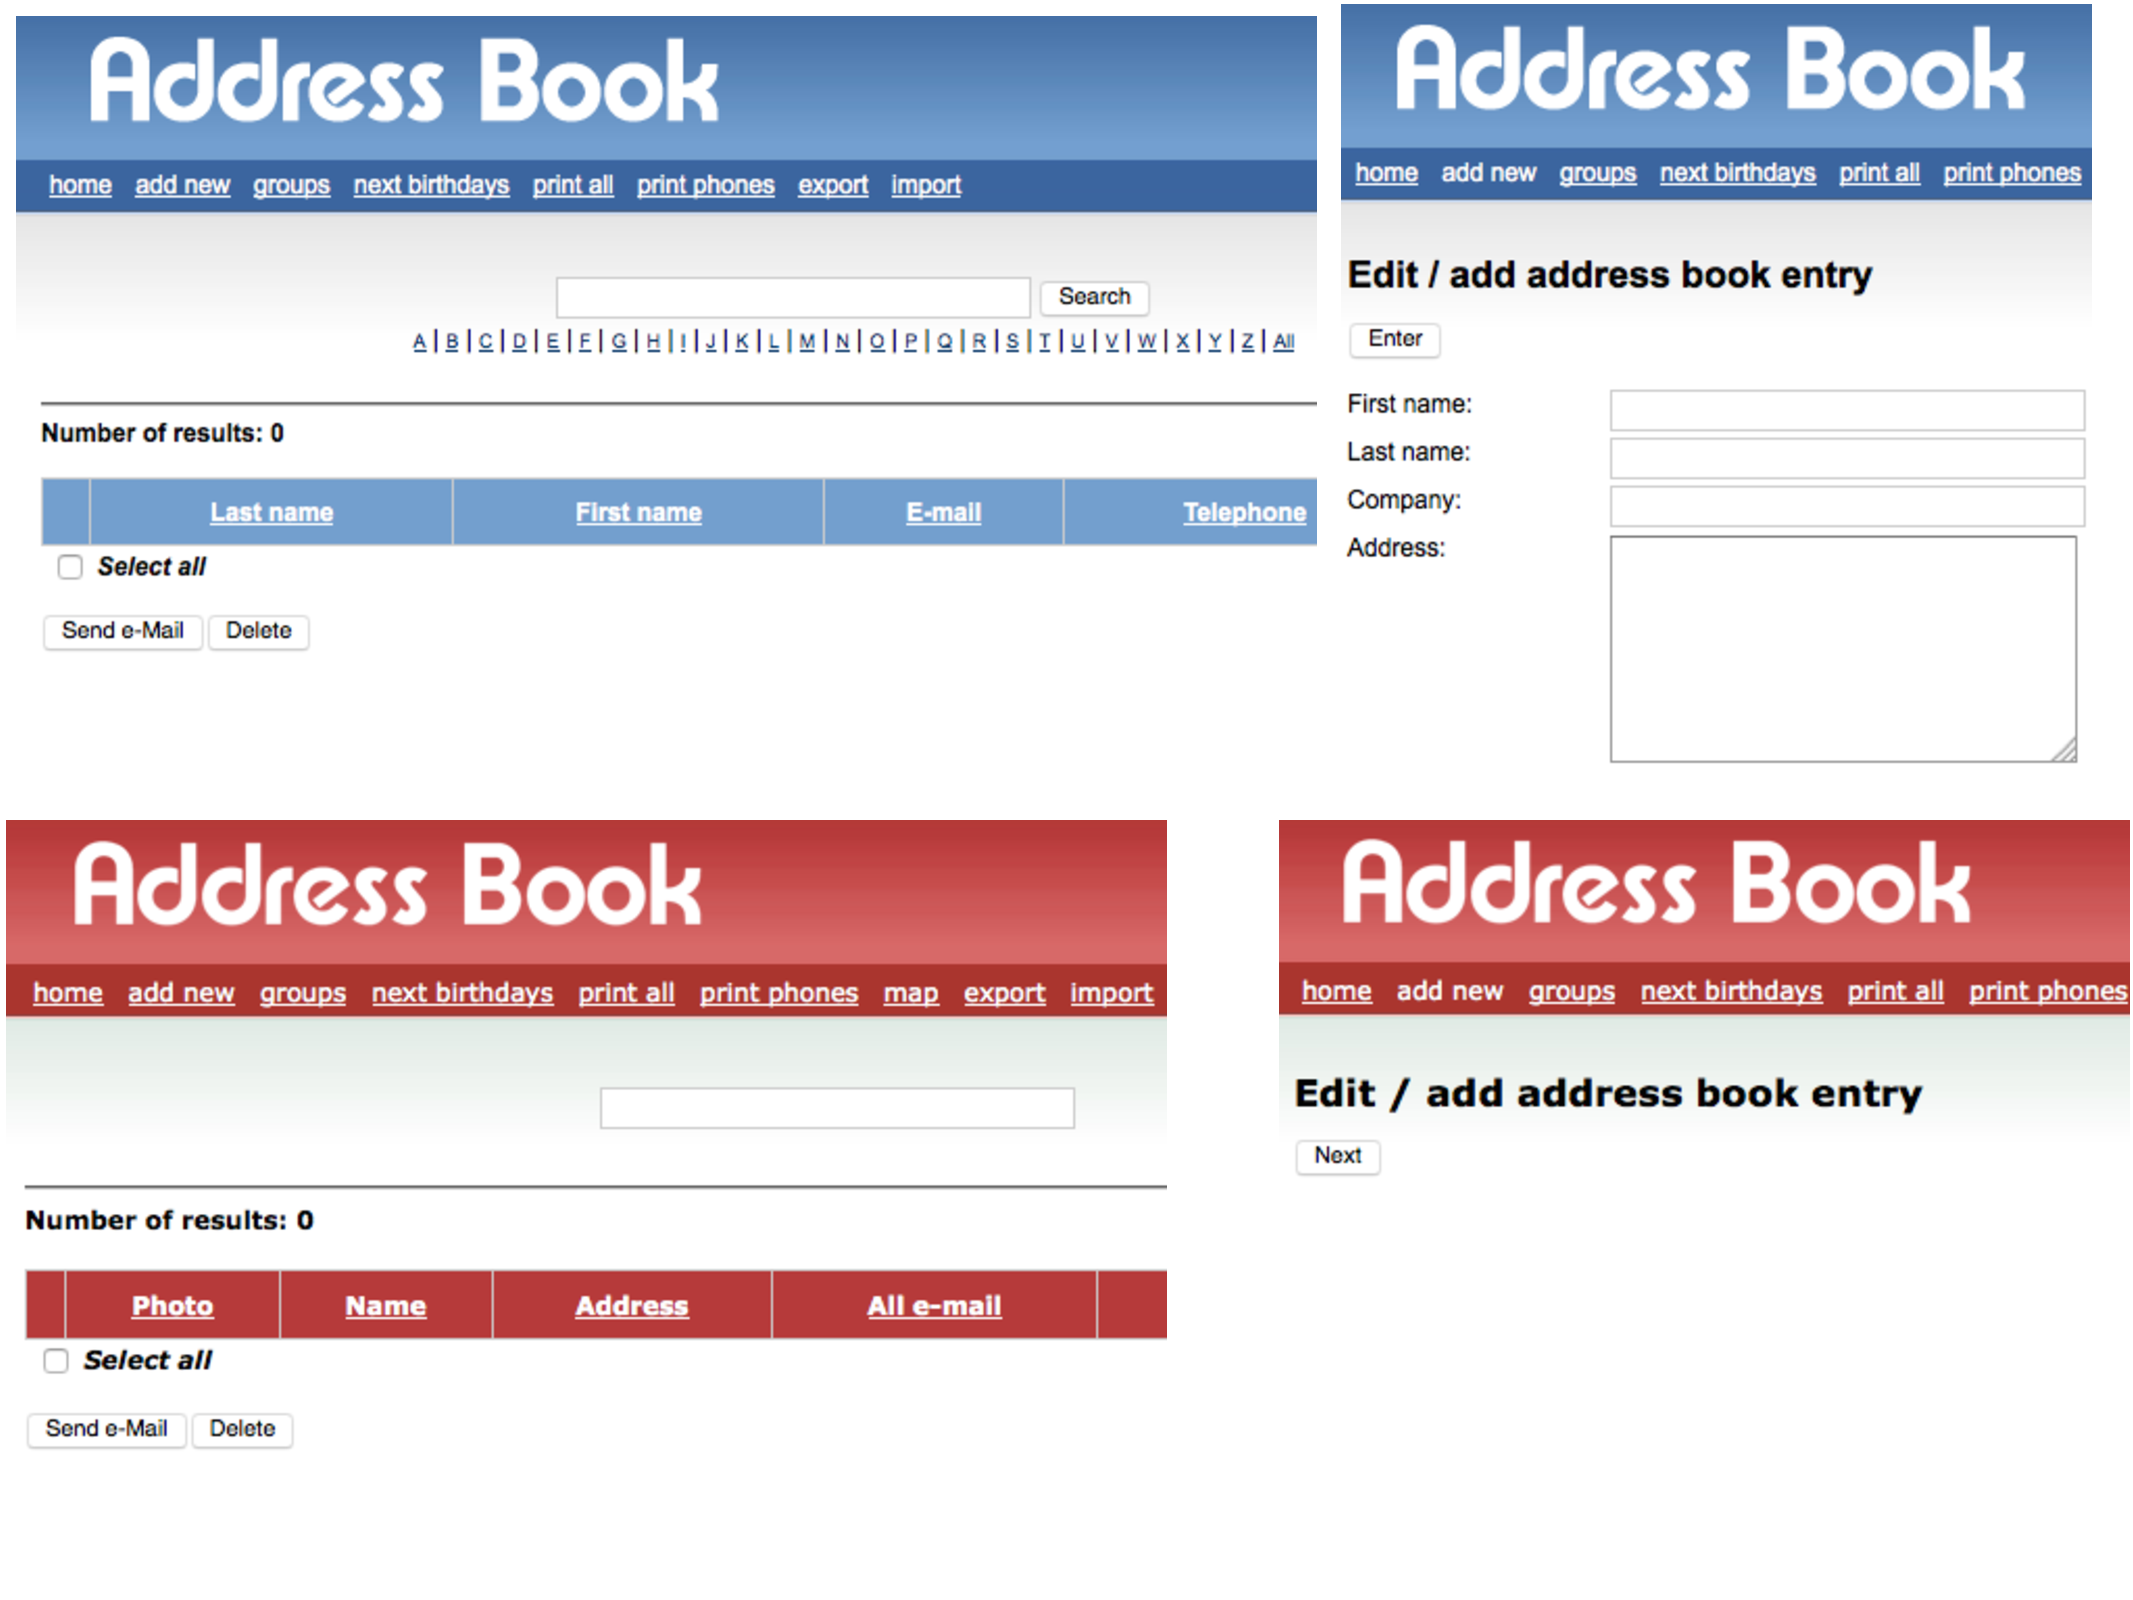
\includegraphics[trim={0cm 2cm 0cm 0cm},clip,scale=0.2]{images/addressbook}
%%%}
%%\caption{AddressBook}
%%\label{addressbook}
%%\end{figure}
%
%\textit{Scenario 2 --- Mis-Selection or Propagated Breakage}.
%We focus on solving the problem due to propagated breakages  because it is very common in web testing due to locators mis-selection. 
%
%We want to make sure that all the locators select the correct elements, respectively.
%
%Two variants: the mis-selection does not cause a state transition (the app remains in the same state), or it does trigger a state transition and leads to a different state.





%% !TEX root =  paper.tex

\section{Breakage Scenarios}\label{sec:study}

Given the predominance of locator-related issues, we focus our analysis on locator problems. We thus conducted a study to categorize the breakages from a repair-oriented perspective. 
While there exist taxonomies related to web and GUI breakages~\cite{Hammoudi-2016-ICST,Issa:2012:VTG:2412102.2412107,7102582}, none of them are detailed enough as far as automatic repair is concerned. 
The findings from this study highlight the complexity and the variety of the breakages that can occur in E2E web tests, and that our approach aims to solve.

\subsection{A repair-oriented test breakages taxonomy}\label{sec:taxonomy}

\head{Study Setting}\label{sec:study}
In the intention of supporting a realistic test regression scenario, we selected open source web applications for which (i)~multiple versions and (ii)~Selenium test cases were available from previous research on web testing~\cite{WCRE}. %Especially the latter requirement was challenging, because non-trivial web test suites are rarely made publicly available, and in fact we found no open-source test suite of reasonable size for our study. Fortunately, we could select four web applications that have been used extensively in the context of previous research on web testing~\cite{WCRE}, and for which we were able to obtain four working Selenium test suites.

\begin{table}[h]
\setlength{\tabcolsep}{2pt}
\renewcommand{\arraystretch}{0.9}
\centering
%\footnotesize
\caption{Subject systems and their test suites}
\begin{tabular}{lrrr@{\hskip 2em}r@{\hskip 1em}r}
\toprule

& \multicolumn{3}{c}{\sc Web Applications} 
& \multicolumn{2}{c}{\sc Test Suites} \\

\cmidrule(r){2-4} \cmidrule(r){5-6}

& {\textbf{Init.}} 
& {\textbf{Rel.}}
& {\textbf{LOCs (K)}} 
& {\textbf{Tot/Avg}} 
& {\textbf{LOCs (K)}}   \\

\midrule
AddressBook   & 4.0       & 47       & 8,757   & 1,344/28        & 61,826/43          \\
Claroline     & 1.10.7    & 11       & 338,129 & 492/41        & 20,287/43          \\
Collabtive    & 0.65      & 13       & 150,696 & 560/40        & 22,710/38          \\
PPMA          & 0.2       & 11       & 556,164 & 276/23        & 16,732/47          \\
\midrule
Total/Average &           & 82       & 263,436 & 2,672/33        & 121,555/43 \\

\bottomrule
\end{tabular}
\label{table:subjectSystems}
\end{table}

\autoref{table:subjectSystems} (Web Applications macro-column) shows information about the selected applications, including their names, the initial release for which the test suites were developed, the numbers of releases available after the initial release, and the number of lines of code (counted using \texttt{cloc}~\cite{cloc} and averaged across the releases).
Test Suites macro-column provides data on the test suites, including the total numbers of test cases counted across all versions along with the average number of test cases per version, and the total numbers of statements in all of the test cases counted across all versions along with the average number of statements per test case.

\head{Procedure}\label{sec:procedure}
First, we determined the types of test breakages that occur in our objects of analysis. For each considered web application, for each version $V_n$ and its accompanying test suite $T_n$, we executed $T_n$ on the subsequent version $V_{n+1}$, and collected information about each breakage and each failure (e.g., actual bugs). We repeated this process until all the versions were taken into account. 

\begin{figure}[t]
\centering
%\fbox{
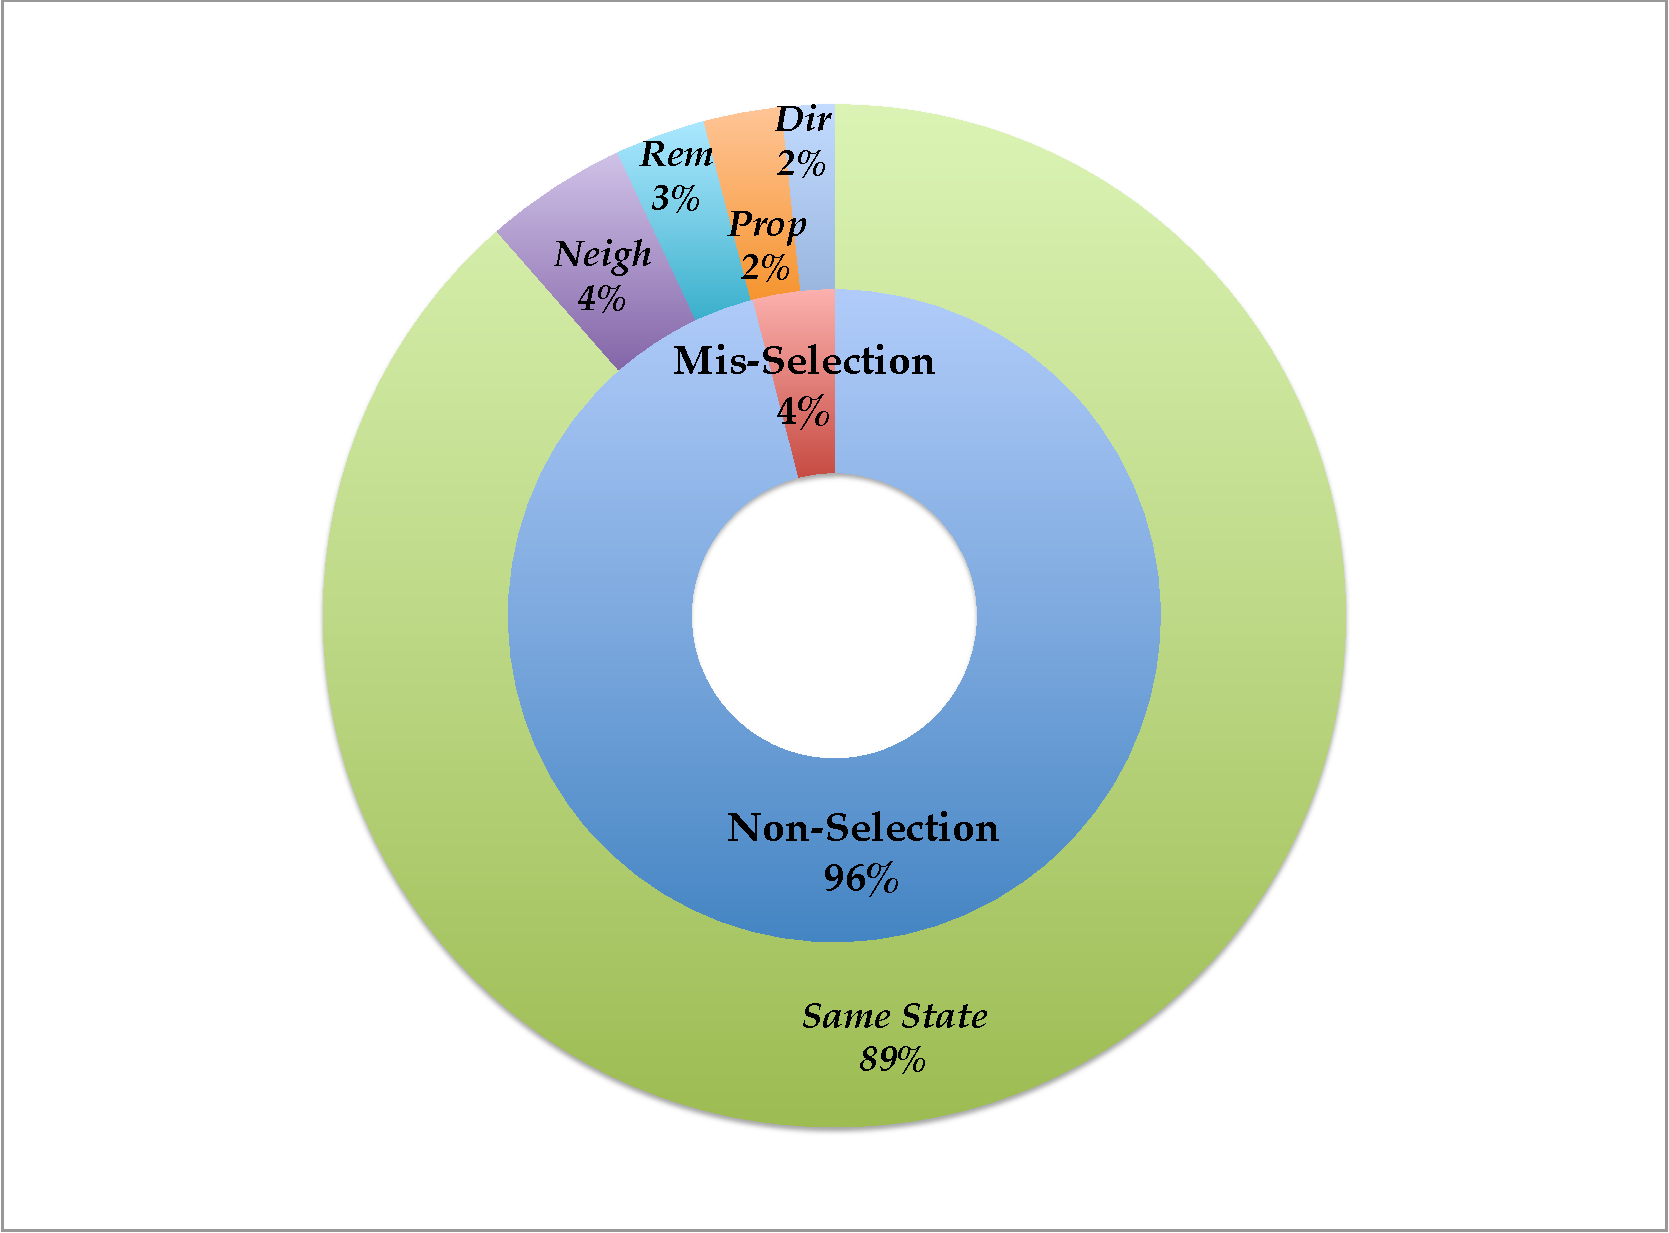
\includegraphics[trim={0cm 0cm 0cm 0cm},clip,scale=0.23]{images/donut}
%}
\caption{Distribution of Different Types of Breakages.}
\label{donut}
\end{figure}

\begin{figure}[b]
\centering
%\fbox{
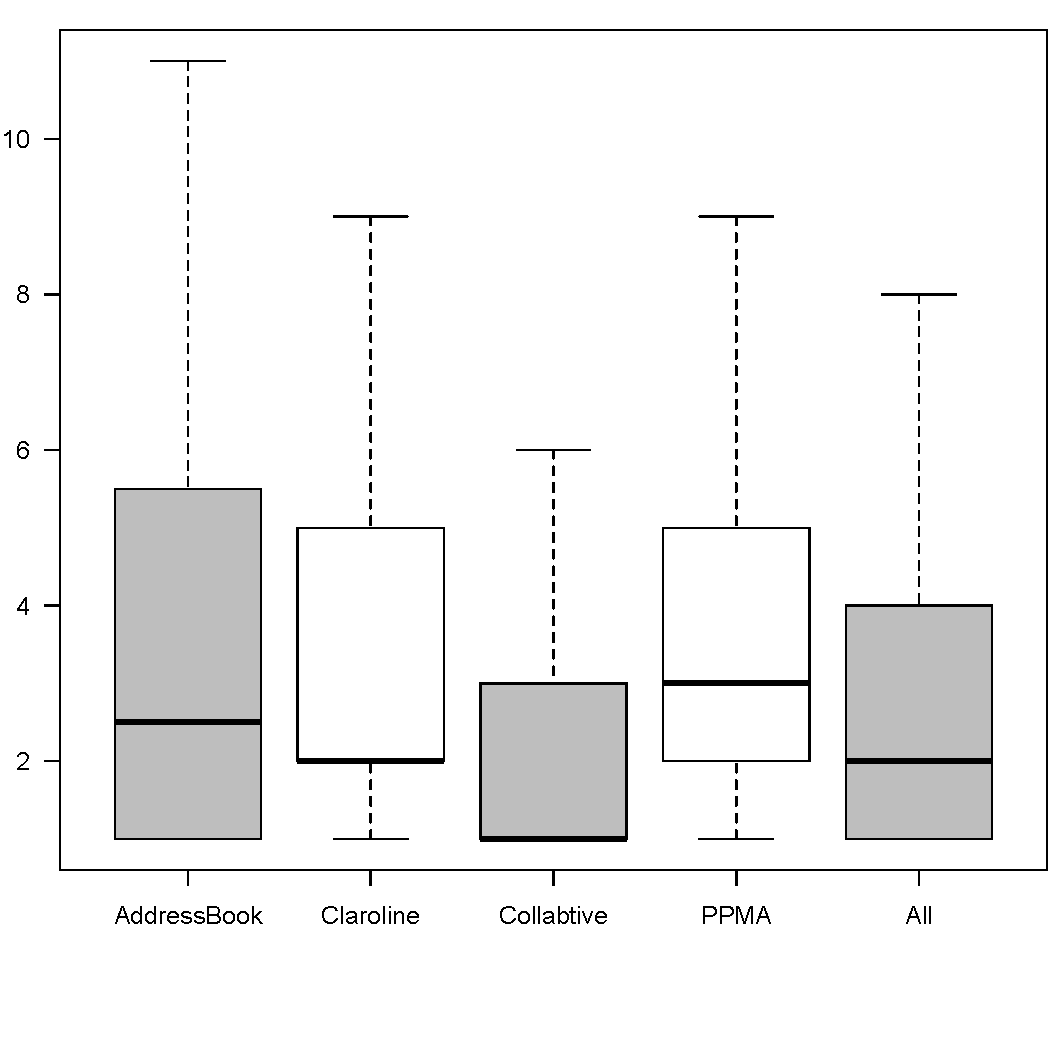
\includegraphics[trim={0cm 0cm 0cm 0cm}, clip,width=0.8\columnwidth]{images/distribution.pdf}
%}
\caption{Distribution of test breakages per test case in each subject system.}
\label{fig:distribution}
\end{figure} 

\begin{figure*}[h!]
\centering
\begin{subfigure}{\columnwidth}
\centering
%\fbox{
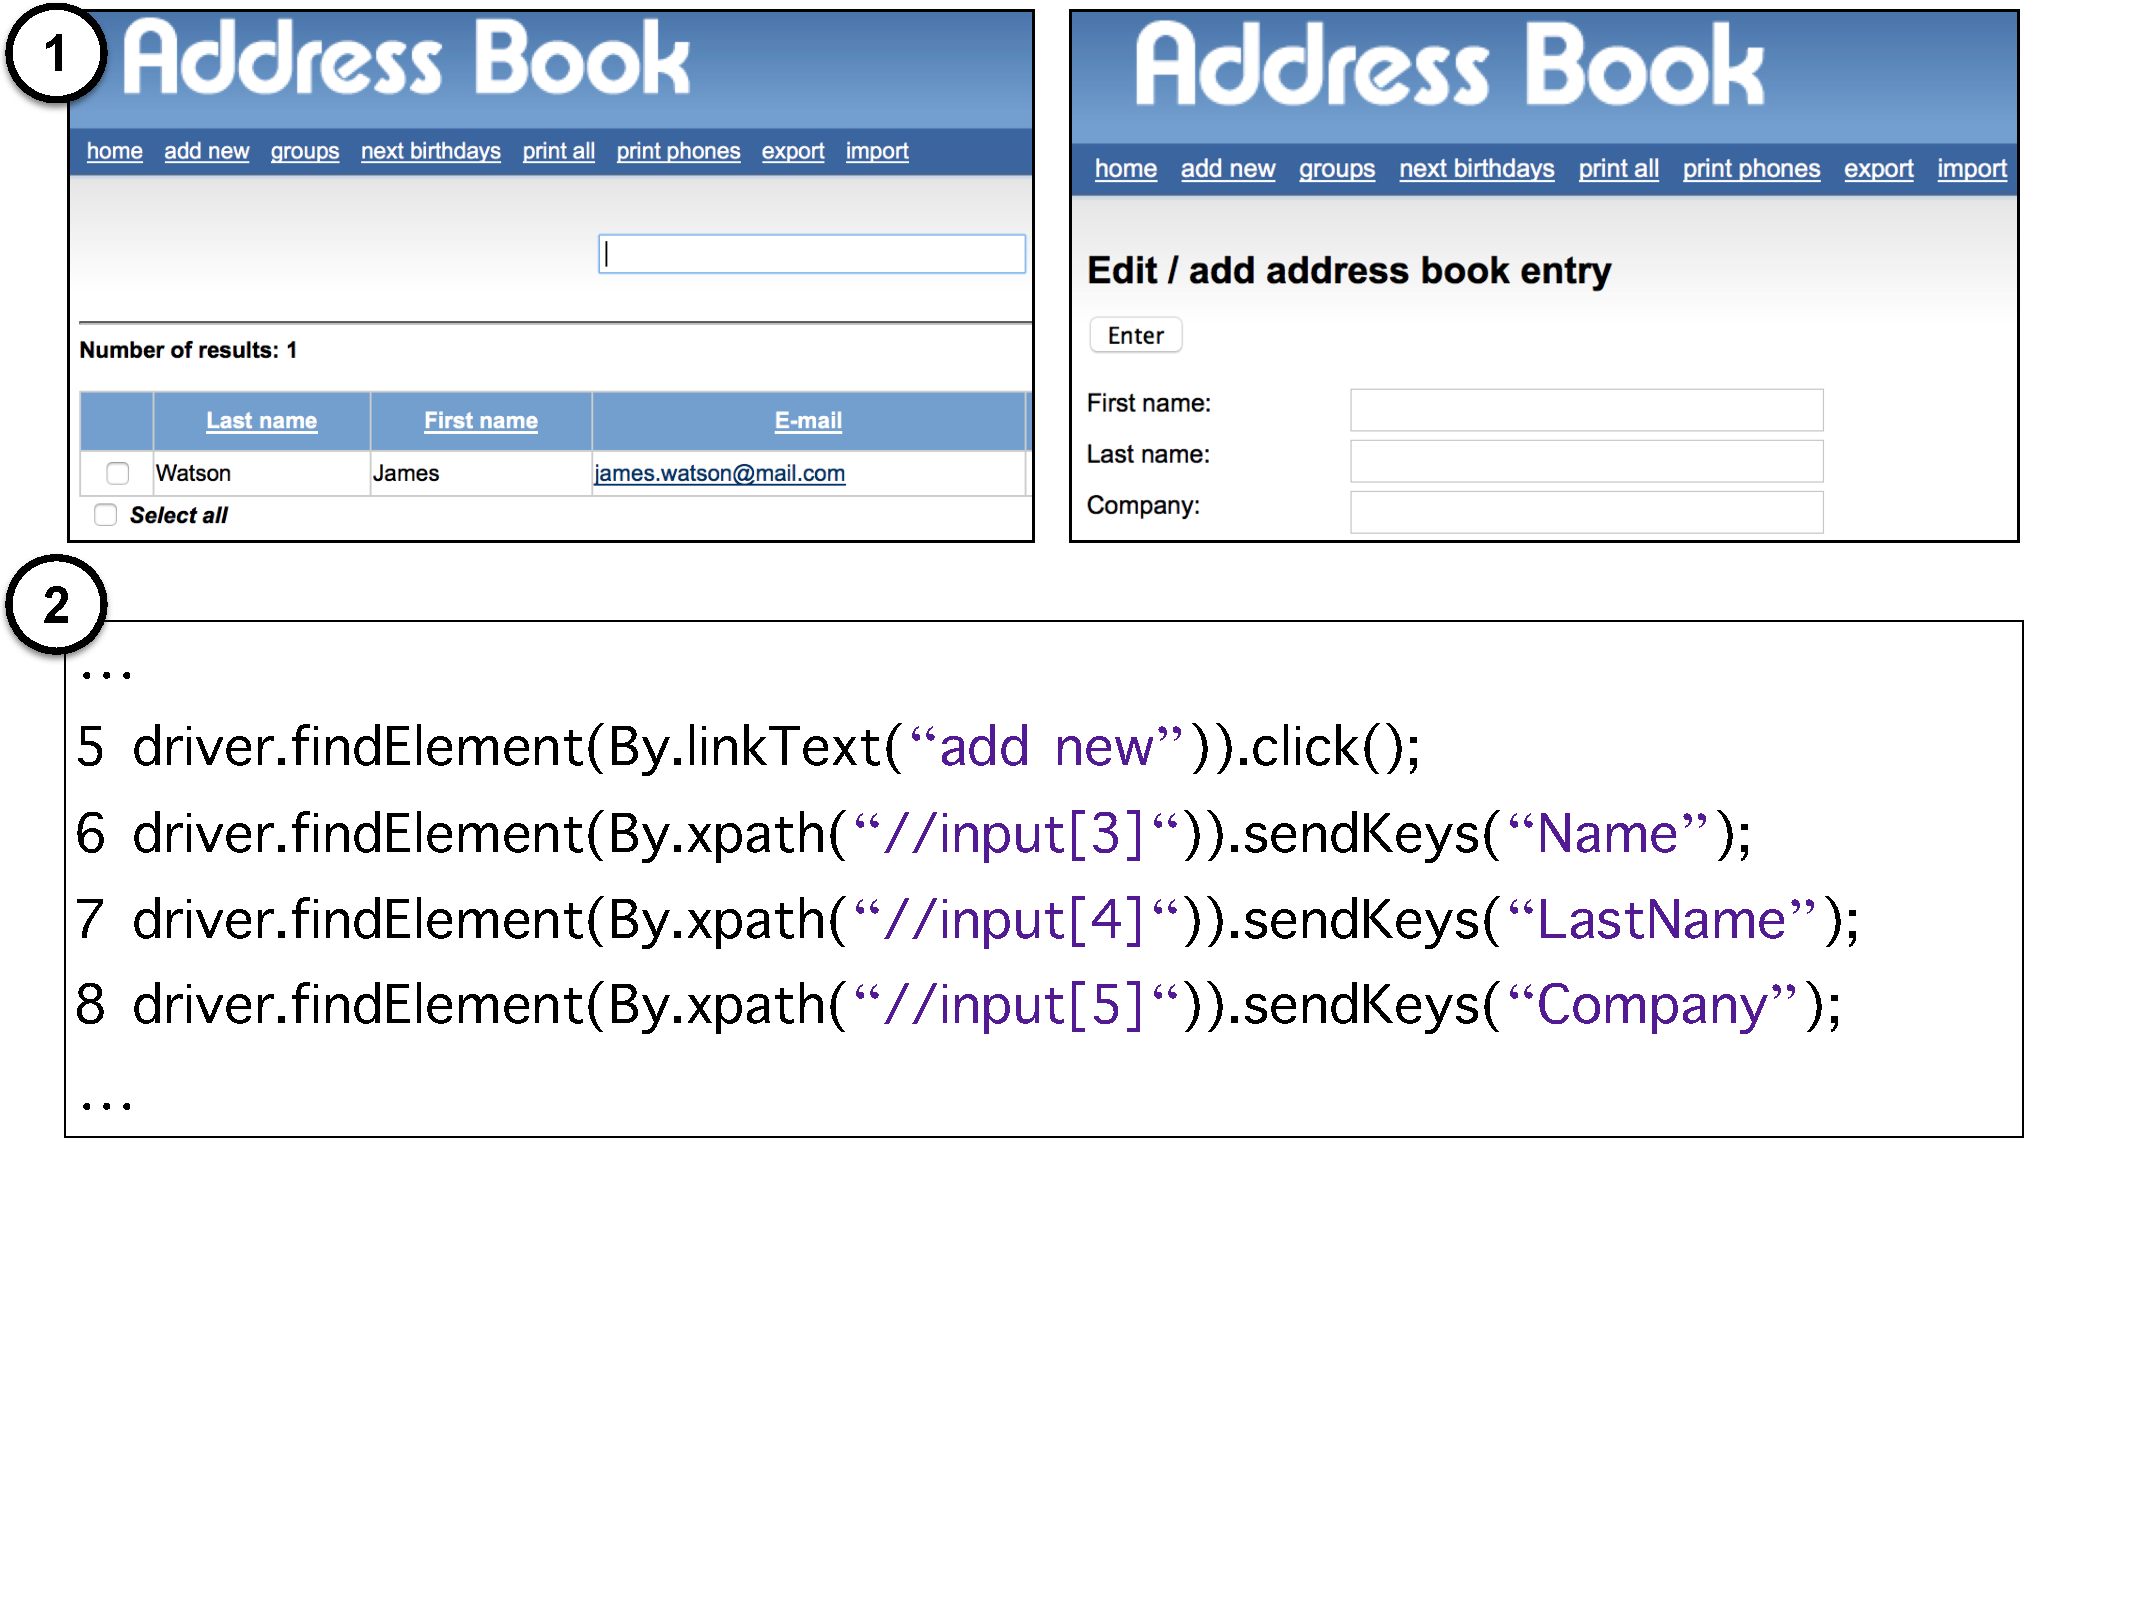
\includegraphics[trim=0cm 6cm 0cm 0cm, clip=true, scale=0.200]{images/addressbook-version1.pdf}
%}
\caption{\emph{Version 6.2.12}}
\label{fig:ab1} 
\end{subfigure}
\begin{subfigure}{\columnwidth}
\centering
%\fbox{
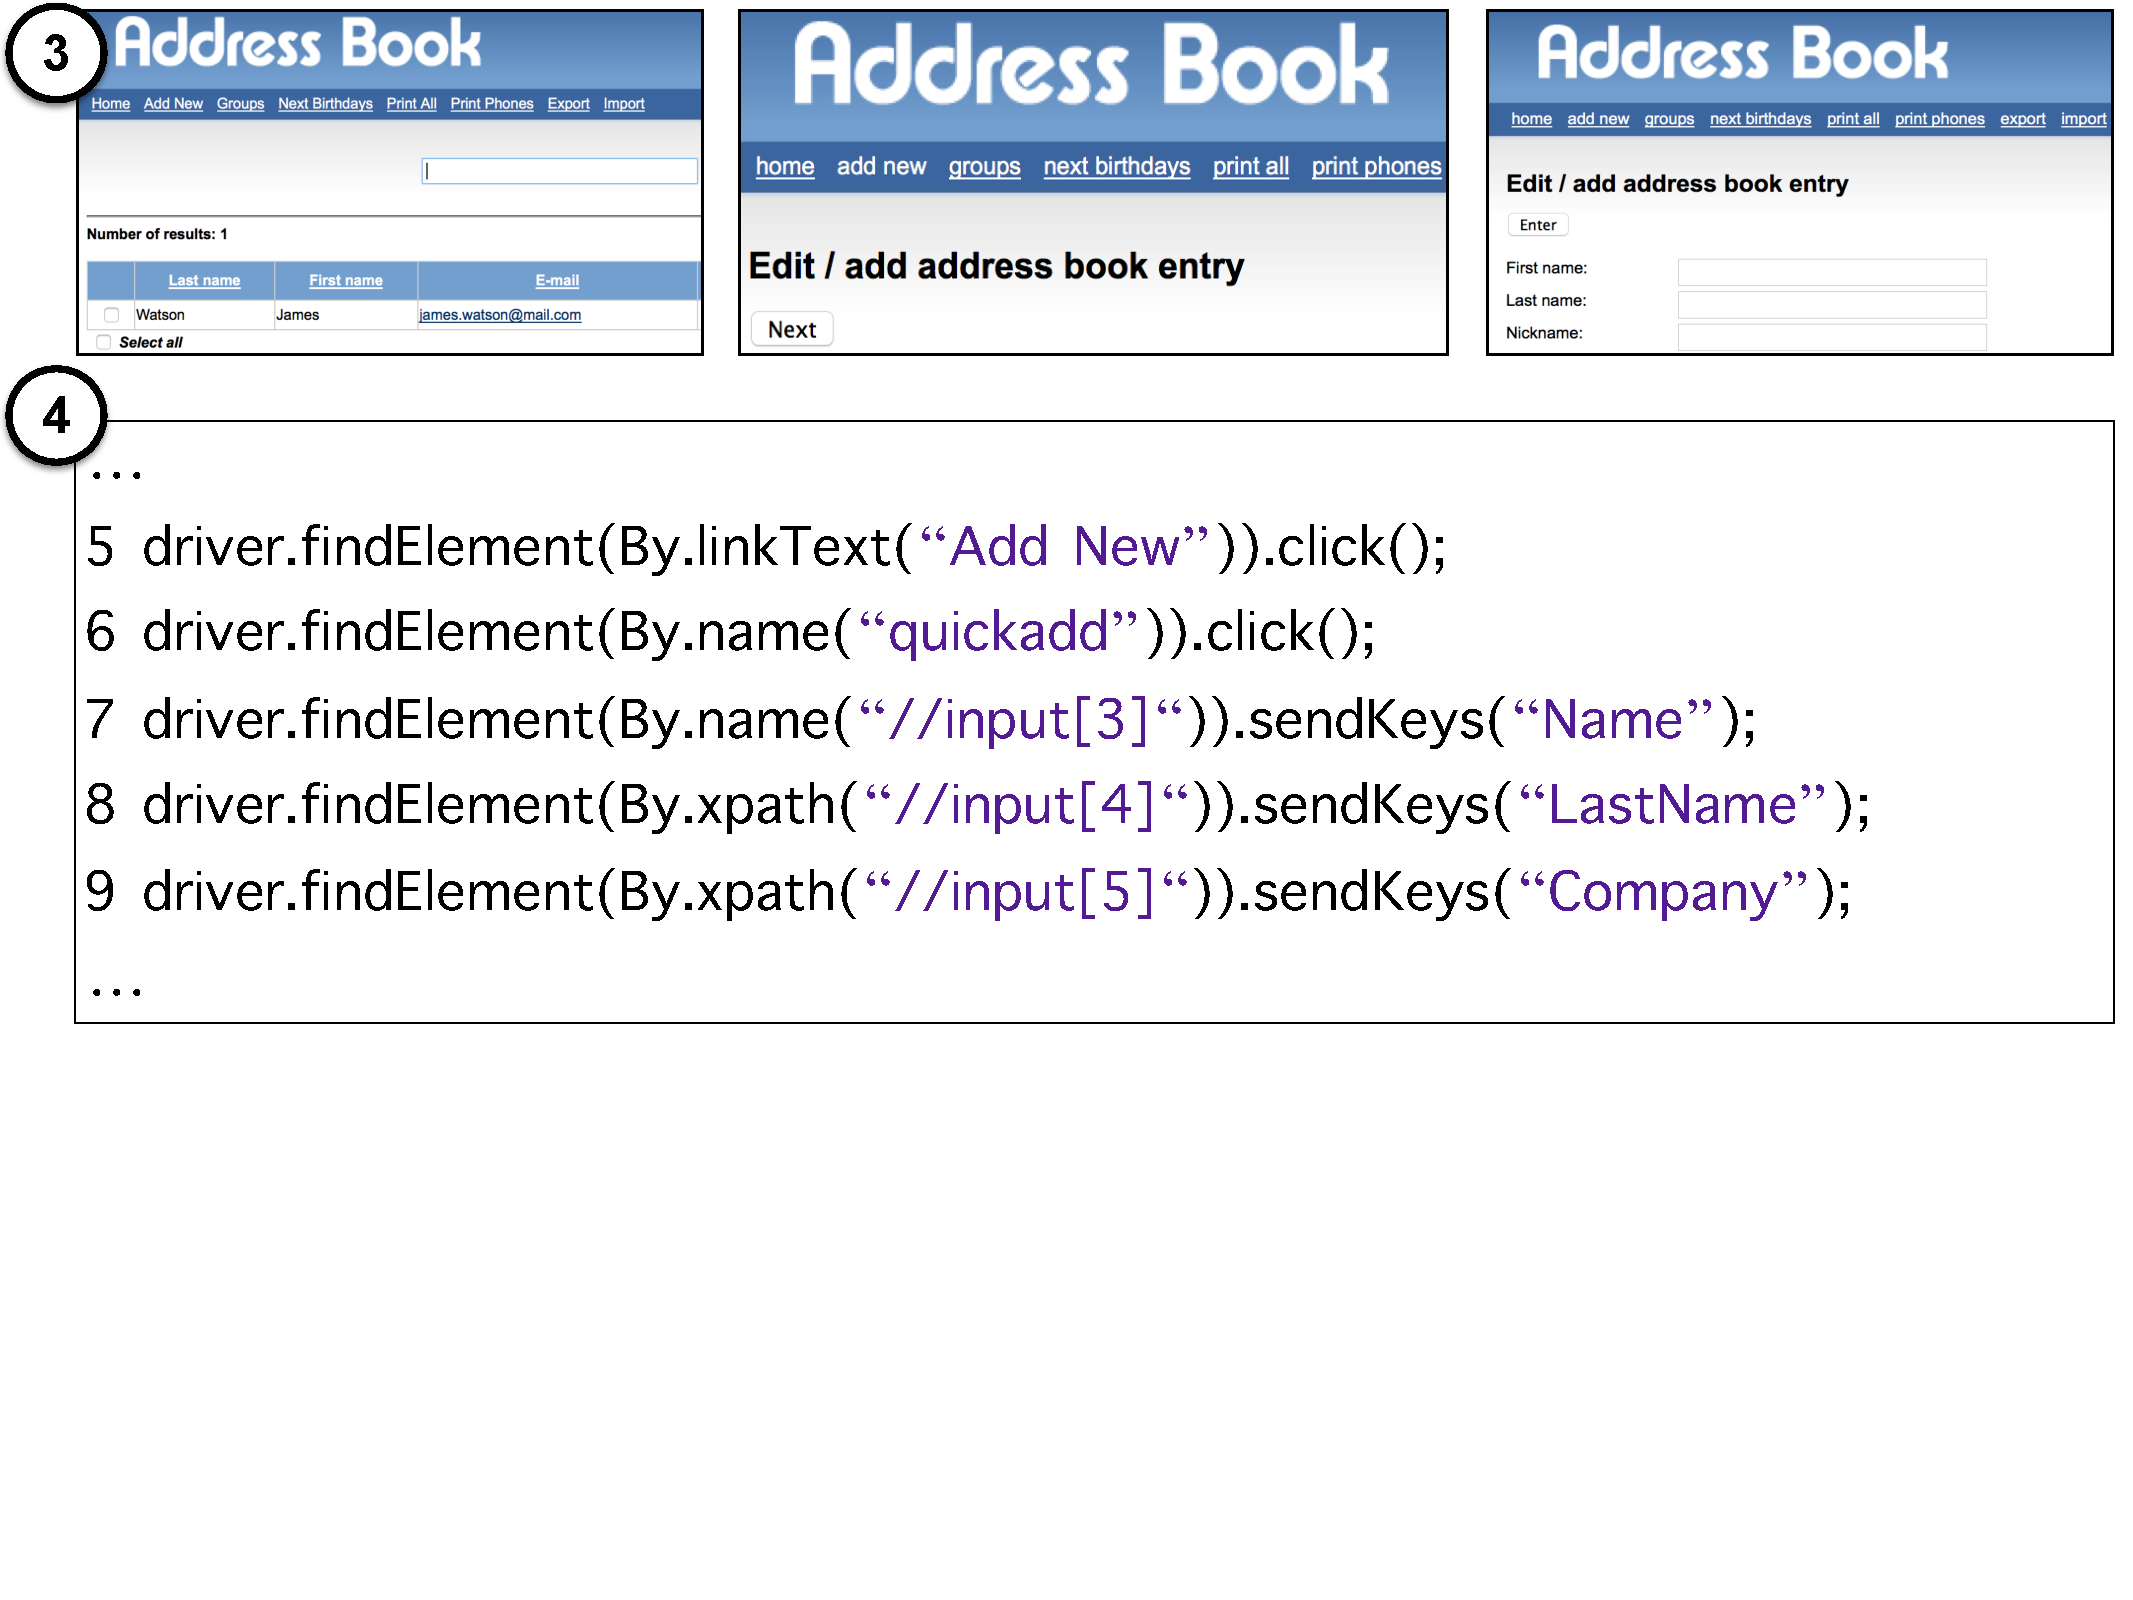
\includegraphics[trim=0cm 5cm 1.3cm 0cm, clip=true,  scale=0.190]{images/addressbook-version2.pdf}
%}
\caption{\emph{Version 7.0.0}}
\label{fig:ab2}
\end{subfigure}
\caption{AddressBook web application, version 6.2.12 (\ref{fig:ab1}) and version 7.0.0 (\ref{fig:ab2}), along with Selenium WebDriver tests.} 
\label{fig:example} 
\end{figure*}

\head{Grounded Theory Study Results}\label{sec:study}
We collected 733 individual test breakages, distributed as follows: 50 for AddressBook, 165 for Claroline, 218 for Collabtive, and 300 for PPMA.
\autoref{donut} shows the distribution of the different types of locator breakages. Our study revealed two major categories, each of which has specific subtypes. The most prevalent category refers to \textit{Non-Selection} of web elements (695/733). Among those, $\approx$93\% are related to web elements that are still on the same web page (or test state), $\approx$5\% pertain to web elements that are moved to a neighbouring web page (or test state), and $\approx$2\% to web elements being removed from any web page.
The second main category consists of \textit{Mis-Selection} of web elements (38/733), of which $\approx$68\% led to \textit{direct} breakages, and $\approx$32\% to \textit{propagated} breakages. 
Additionally, we collected 94 test \textit{failures}---meaning the tests exposing actual bugs---and 22 failures due to obsolete \textit{assertion} values.
%
That said, in the context of this paper, we focus on repairing the regression breakages. 

\autoref{fig:distribution} shows box-plots about the distribution of breakages per test cases in each subject system. We observe that on average between 1--4 breakages are present per test. 
In short, (1)~test suites tend to break frequently as the web application evolves, and (2)~breakages may pertain occur multiple times within the same test. 
In the following of this section, we detail the test breakage scenarios by means of a running example.

\subsection{Breakage Scenarios}\label{sec:breakage-scenarios}

\noindent
\textbf{Basic Terminology.}
At a high level, each web test statement is a tuple \textit{<locator, action, value>}. 
The locator component specifies the web element the test statement is interacting with. A locator is a function on a DOM state $\mathcal{D}$. Notationally, $l: \mathcal{D} \rightarrow \{e\}$ where $e$ is the web element returned by the locator $l$ when applied to $\mathcal{D}$. 
%
%Locator breakages are due to one or more DOM-based root causes. A root cause is a tuple $<\mathcal{D}, e, a, v>$ where $\mathcal{D}$ is a DOM tree (e.g., a test state), $e$ is the web element in $\mathcal{D}$ on which the test currently operates, $a$ is a HTML attribute of $e$, and $v$ is the value of $a$. 
%We define a repair as a tuple $<r, e', a', v', \mathcal{D'}>$, where $r$ is a root cause and $e'$ is the suggested new web element for $\mathcal{D}$ in the root cause $r$, having attribute $a'$ set to $v'$. 
%The locator function is surjective, that is every web element $e$ is mapped to by at least one locator (e.g., the XPath from the root to $e$), but there exist multiple locators {$\displaystyle \forall l\in L,\exists e\in D{\text{ such that }} l: D \rightarrow \{e\}$}.



\noindent
\textbf{Scenario 1 (Non-Selection $\bullet$ Same State).}
A non-selection occurs when a locator $l$ applied to a DOM state $\mathcal{D}$ returns no elements---formally, $l: \mathcal{D} \rightarrow \emptyset$, but the target element $e$ is still present on the page ($e \in \mathcal{D}$).
Then, possible repairs require to find another locator $l' \mid l': \mathcal{D} \rightarrow e$.

As an example, consider the login page of AddressBook in~\autoref{fig:ab1}~\textcircled{\raisebox{-0.8pt}{1}}, and the accompanying WebDriver test~\textcircled{\raisebox{-0.8pt}{2}}. 
%, which was developed for (or evolved until) version 6.2.12, where it runs correctly.
%\textcircled{\raisebox{-0.8pt}{1}}~shows the home page of AddressBook web application version 6.2.12, and the page in which the user can insert a new entry. A portion of a possible Selenium WebDriver test script is also shown~\textcircled{\raisebox{-0.8pt}{2}}, which was developed for (or evolved until) version 6.2.12, where it runs correctly.
%
Suppose that in the new subsequent version of AddressBook (7.0.0), as a result of the application evolution, 
the login button gets modified as follows: \code{<input value=``Login''></input>} becomes \code{<button>Login</button>}.
%\texttt{id=``submitLogin''}. In particular, the menu bar items have been capitalized, and a new confirmation page has been added before the insert entry page. 
%Finally,~\textcircled{\raisebox{-0.9pt}{4}} shows a portion of a Selenium WebDriver test~\cite{selenium} which fills in the username and password input boxes (Lines~5-6), and submits the form (Line~7). Suppose the test was developed for (or evolved until) version 1.10.0, where it ran correctly.

When executed on version 7.0.0, the test~\textcircled{\raisebox{-0.8pt}{2}} will then stop at Line~4 when attempting to locate the login button. %Non-selection problems manifest as \textit{direct} breakages, because the broken statement is the one that needs to be repaired.  
%
At a visual inspection of the two GUIs, a tester would expect the test to work, because her perception is immaterial where changes at DOM-level are concerned. It is indeed evident that the target element is \textit{visually} still present on the page, and its position \textit{on the GUI} has not changed.
 

%At this aim, a tester may wish to use the \water  technique~\cite{Choudhary:2011:WWA:2002931.2002935} to automatically repair the broken statement. Specifically, another locator for the ``Login'' button needs to be found, rather the relying on ``broken'' \texttt{value} attribute. \water will attempt to gather information about the broken element (such as the XPath, and the various attributes) by analysing the DOM of the previous version, and match such information on the evolved DOM of version 7.0.0. Unfortunately, \water's technique is ineffective in such a scenario, because (1)~the attribute \texttt{value} has been deleted from the DOM, and (2)~the XPath and the tag of the target element have changed (from \mbox{\texttt{input}} to \mbox{\texttt{button}}), which renders impossible for \water's heuristic to identify it on the evolved DOM. 
 
%\noindent
%\textit{Visual-aided Mitigation.}
%In this case, an algorithm taking into consideration the visual appearance of the test state might be able to match the target element between the two GUIs (in a similar way as a human would do). However, this task is challenging to be automated because several issues needs first to be solved. Among all (1)~finding an accurate visual matching technique, and, in the case a visual match is found, (2)~retrieving the corresponding element in the DOM. 

\noindent
\textbf{Scenario 2 (Non-Selection $\bullet$ Neighbouring State).}
Notationally this can be expressed as $l: \mathcal{D} \rightarrow \emptyset \land \exists \ \mathcal{D'} \mid l: \mathcal{D'} \rightarrow \{e\}$.
As a concrete example consider \autoref{fig:ab1}~\textcircled{\raisebox{-0.7pt}{1}}, %showing Addressbook web application version 6.2.12, 
specifically the pages in which the user can insert a new entry. The test~\textcircled{\raisebox{-0.7pt}{2}} clicks on the ``add new'' link on the home page (Line~5), and fills in the ``First name'', ``Last name'' and ``Company'' text fields (Lines~6--8).
Suppose now to replay the test on the successive version 7.0.0~\textcircled{\raisebox{-0.7pt}{3}}, for regression purposes. The test will raise an exception of kind \texttt{NoSuchElementException} at Line~6, when attempting to locate the ``First name'' text field~\textcircled{\raisebox{-0.7pt}{2}}. 
Indeed, a new intermediate confirmation page has been added~\textcircled{\raisebox{-0.9pt}{3}}, and the navigational workflow of the test must be corrected to reflect that of the new  web application.

From a testing perspective, the ``First name'' text field can no longer be found on the web page (test state) following the execution of the statement at Line~5. However, conceptually, the repair action that needs to be triggered in order to correct the test has nothing to do with the locator at Line~6.
In fact, by only looking at the exception, it is arduous for the tester to understand what the actual problem is, unless the \textit{visual execution} of the test is taken into consideration.
%
%Even the use of \water is unsuccessful, because it would attempt at repairing the broken statement at Line~6. (the technique only handles addition of statements within forms, and does not apply to general broken workflow scenarios).
%
%\noindent
%\textit{Visual-aided Mitigation.}
A possible solution would require to (1)~detect that the web element $e$ no longer exists as part of the test state $st_i$ in version $V$, (2)~try to match the $e$ in one of the neighbouring states of $st_i$ in the new version $V'$, which requires to (3)~find  a web element $e' \in st_i$ such that $(e', st_i) \rightarrow st_j$ (the ``Next'' button in our example~\textcircled{\raisebox{-0.7pt}{3}}).

\noindent
\textbf{Scenario 3 (Non-Selection $\bullet$ Removed).} 
%
The third and last \textit{Non-Selection} scenario concerns a web element being deleted from a web page. Formally, $l: \mathcal{D} \rightarrow \emptyset \land \nexists \ \mathcal{D'} \mid l: \mathcal{D'} \rightarrow \{e\}$.
In a way, this can be seen as the opposite scenario of Scenario 2. 
As a concrete example, consider the example of \autoref{fig:ab2}, with the application being evolved in the reverse order as depicted in the figure (thus considering going from version 7.0.0 to version 6.2.12). The test~\textcircled{\raisebox{-0.7pt}{4}} would stop at Line 6, when trying to select the ``Next'' button, which was on a page that is no longer present. In this case, the only possible fix is to delete the statement.

%\noindent
%\textit{Visual-aided Mitigation.}
%A possible solution would require to (1)~search for the the web element $e$ both in $st_i$ and its neighbouring states, and (2)~if not match is found, then remove the statement.

\noindent
\textbf{Scenarios 4 and 5 (Mis-Selection $\bullet$ Direct and Propagated).}\label{sec:misselection}
Problems occur not only when web elements are being deleted, but also when they get modified, either in their position on the DOM tree, or in their position in the application state space. This can cause tests to ``mis-select'' elements.
Specifically, a mis-selection occurs when a locator selects a different DOM element from the one that was used to target. 
%Suppose having version $V$ and a test $t$, composed of a statement $st_i$, which uses a locator $l$ (where $l: \mathcal{D} \rightarrow \{e\}$). In the next version $V'$, $l: \mathcal{D}' \rightarrow \{e'\}$ where $e \ne e'$.
Notationally, $l: \mathcal{D} \rightarrow \{e\}$ in $V$, and $l: \mathcal{D}' \rightarrow \{e'\}$ in $V'$ where $e \ne e'$.
%A mis-selection of an element can lead to unpredictable misbehaviours of the test, being responsible of either direct or propagated breakages.

Consider \autoref{fig:example} again. 
Suppose that the test~\textcircled{\raisebox{-0.9pt}{2}} is repaired so as to reach the edit page on version 7.0.0 (for instance, as in~\textcircled{\raisebox{-0.9pt}{4}}). On the new version 7.0.0, the statements at Lines~6--7 will execute correctly, whereas at Line~8 (which will be Line~9 in the new version) will fill in the field ``Nickname'', instead of the field ``Company''.

The mis-selection problem can lead to unpredictable test executions, that diverge from the test's intended behaviour. Depending on the kind of actions, the test execution might result in a \textit{direct}, \textit{propagated} or silent breakage~\cite{Hammoudi-2016-ICST}. Thus, the point in which the repair must be applied varies depending on where the mis-selection originated. (The test may continue its execution until it reaches a point in which an action cannot be performed or an element cannot be found, but the actual repair has to be triggered \textit{in a previous test statement}).
Repairing mis-selections requires to find another locator $l' \mid l': \mathcal{D'} \rightarrow \{e\}$.
%\noindent
%\textit{Visual-aided Mitigation.}
%A possible solution would require to (1)~visually validate that the web element $e$ is still targeting the correct element in the new version and (2)~try to correct it, otherwise.

\noindent
\textbf{Summary.}
We have discussed five (5) test breakage scenarios from a repair-oriented standpoint. It is worth remarking, however, that the presented scenarios can also occur together in the same test (i.e., \textit{multiple} breakages). We do not claim that such a list represents all the possible scenarios. However, this list has been found empirically after running several hundreds of tests on real-size applications. 

%\head{How Testers Repair}
%%
%%When a test $t$ that was used to function on a version $V$  breaks on a successive version $V'$, a tester needs to understand the root cause behind the breakage and a possible repair for it. 
%%
%When a test $t$ breaks, at least four steps are involved. 
%(1)~The tester inspects the error stack trace or the console, which may contain information about the origin of breakage (e.g., ``\texttt{NoSuchElementException} occurred. Unable to locate element with \mbox{\texttt{name=password}}''). 
%(2)~The tester uses the message to inspects $t$ looking for the statement $st$ responsible for the failure. %which is also likely to be the one that needs to be corrected (note that this is not always true).
%(3)~The tester navigates the GUI of $V'$, trying to identify the portion of the GUI related to $st$. 
%(4)~The tester inspects either the DOM, or the GUI, or both the DOM and the GUI of $V'$ to find candidate repair solutions. In doing so, the tester may possibly need to exercise manually the same broken scenario of $t$ (i.e., all the actions in the statements preceding $st$), in order to replicate the breakage occurred at $st$ and gather insights on possible repair actions.
%
%To wrap up, a \textbf{first challenge} in repairing web tests derives from the fact that  
%%Thus, in E2E web tests such as Selenium's 
%the tester often needs to inspect and link the behaviour of the test code execution, to the modification perpetrated to the GUI and the DOM of the application. 
%In other words, breakages are often repaired by finding candidate solutions through the inspection of the DOM and the GUI \textit{at the same time}.
%For this reason, it is arguably more difficult to repair Selenium's tests than standard JUnit tests for desktop applications (for which the error messages are typically more informative and IDE features make the debugging activities easier).
%%
%A \textbf{second challenge} is related to the time needed to find and correct the breakages, which may be significantly high~\cite{Leotta-TAIC-2013,JAMAICA2013}. One of the main reasons is due to the low support by the existing test automation tools in understanding the root causes behind test breakages and how they do relate with the changes made in the web applications. 
%
%In this paper we wish to make step ahead to provide such understanding. 
%Our aim is to combine the knowledge present in the DOM of the application with its visual appearance, so as to effectively aid the tester in detecting and repairing test breakages or in validating their correctness. %Our approach aims at automating the mental model the testers create when a test case is executed against a web application GUI. In our belief, such a model is a viable means for automating test case repair.

%Existing locator repair techniques are indeed limited when the web application undergoes drastic structural changes because they only consider the DOM as source where to find possible repairs.
%However, we argue that visual image recognition can help verify each test step (i.e., locator), signalling and fixing the breakages that pertain to locators.




%% !TEX root =  paper.tex
\section{Approach}\label{sec:approach}

The goal of our approach is to find potential fixes that can repair a broken web test that used to work correctly on a version $V$ of the AUT, and that now breaks when applied on a subsequent version $V+n$ (with usually $n=1$).

The focus of our technique is to repair \textit{locators}, that represent the main source of breakage.
Our technique can detect and correct locator problems that pertain to the breakage scenarios described in \autoref{sec:breakage-scenarios}.
In a nutshell, we capture the execution trace of each test statement for a version $V$ and use it to assert the correctness of the test execution and repair it for a subsequent version $V+n$. While for certain breakages, we automatically repair them, we also warn the developer of potential inconsistencies or breakages, and creates potential candidate repairs that fix them. \andrea{suggest vs repair}

\begin{figure}[t]
\centering
%\fbox{
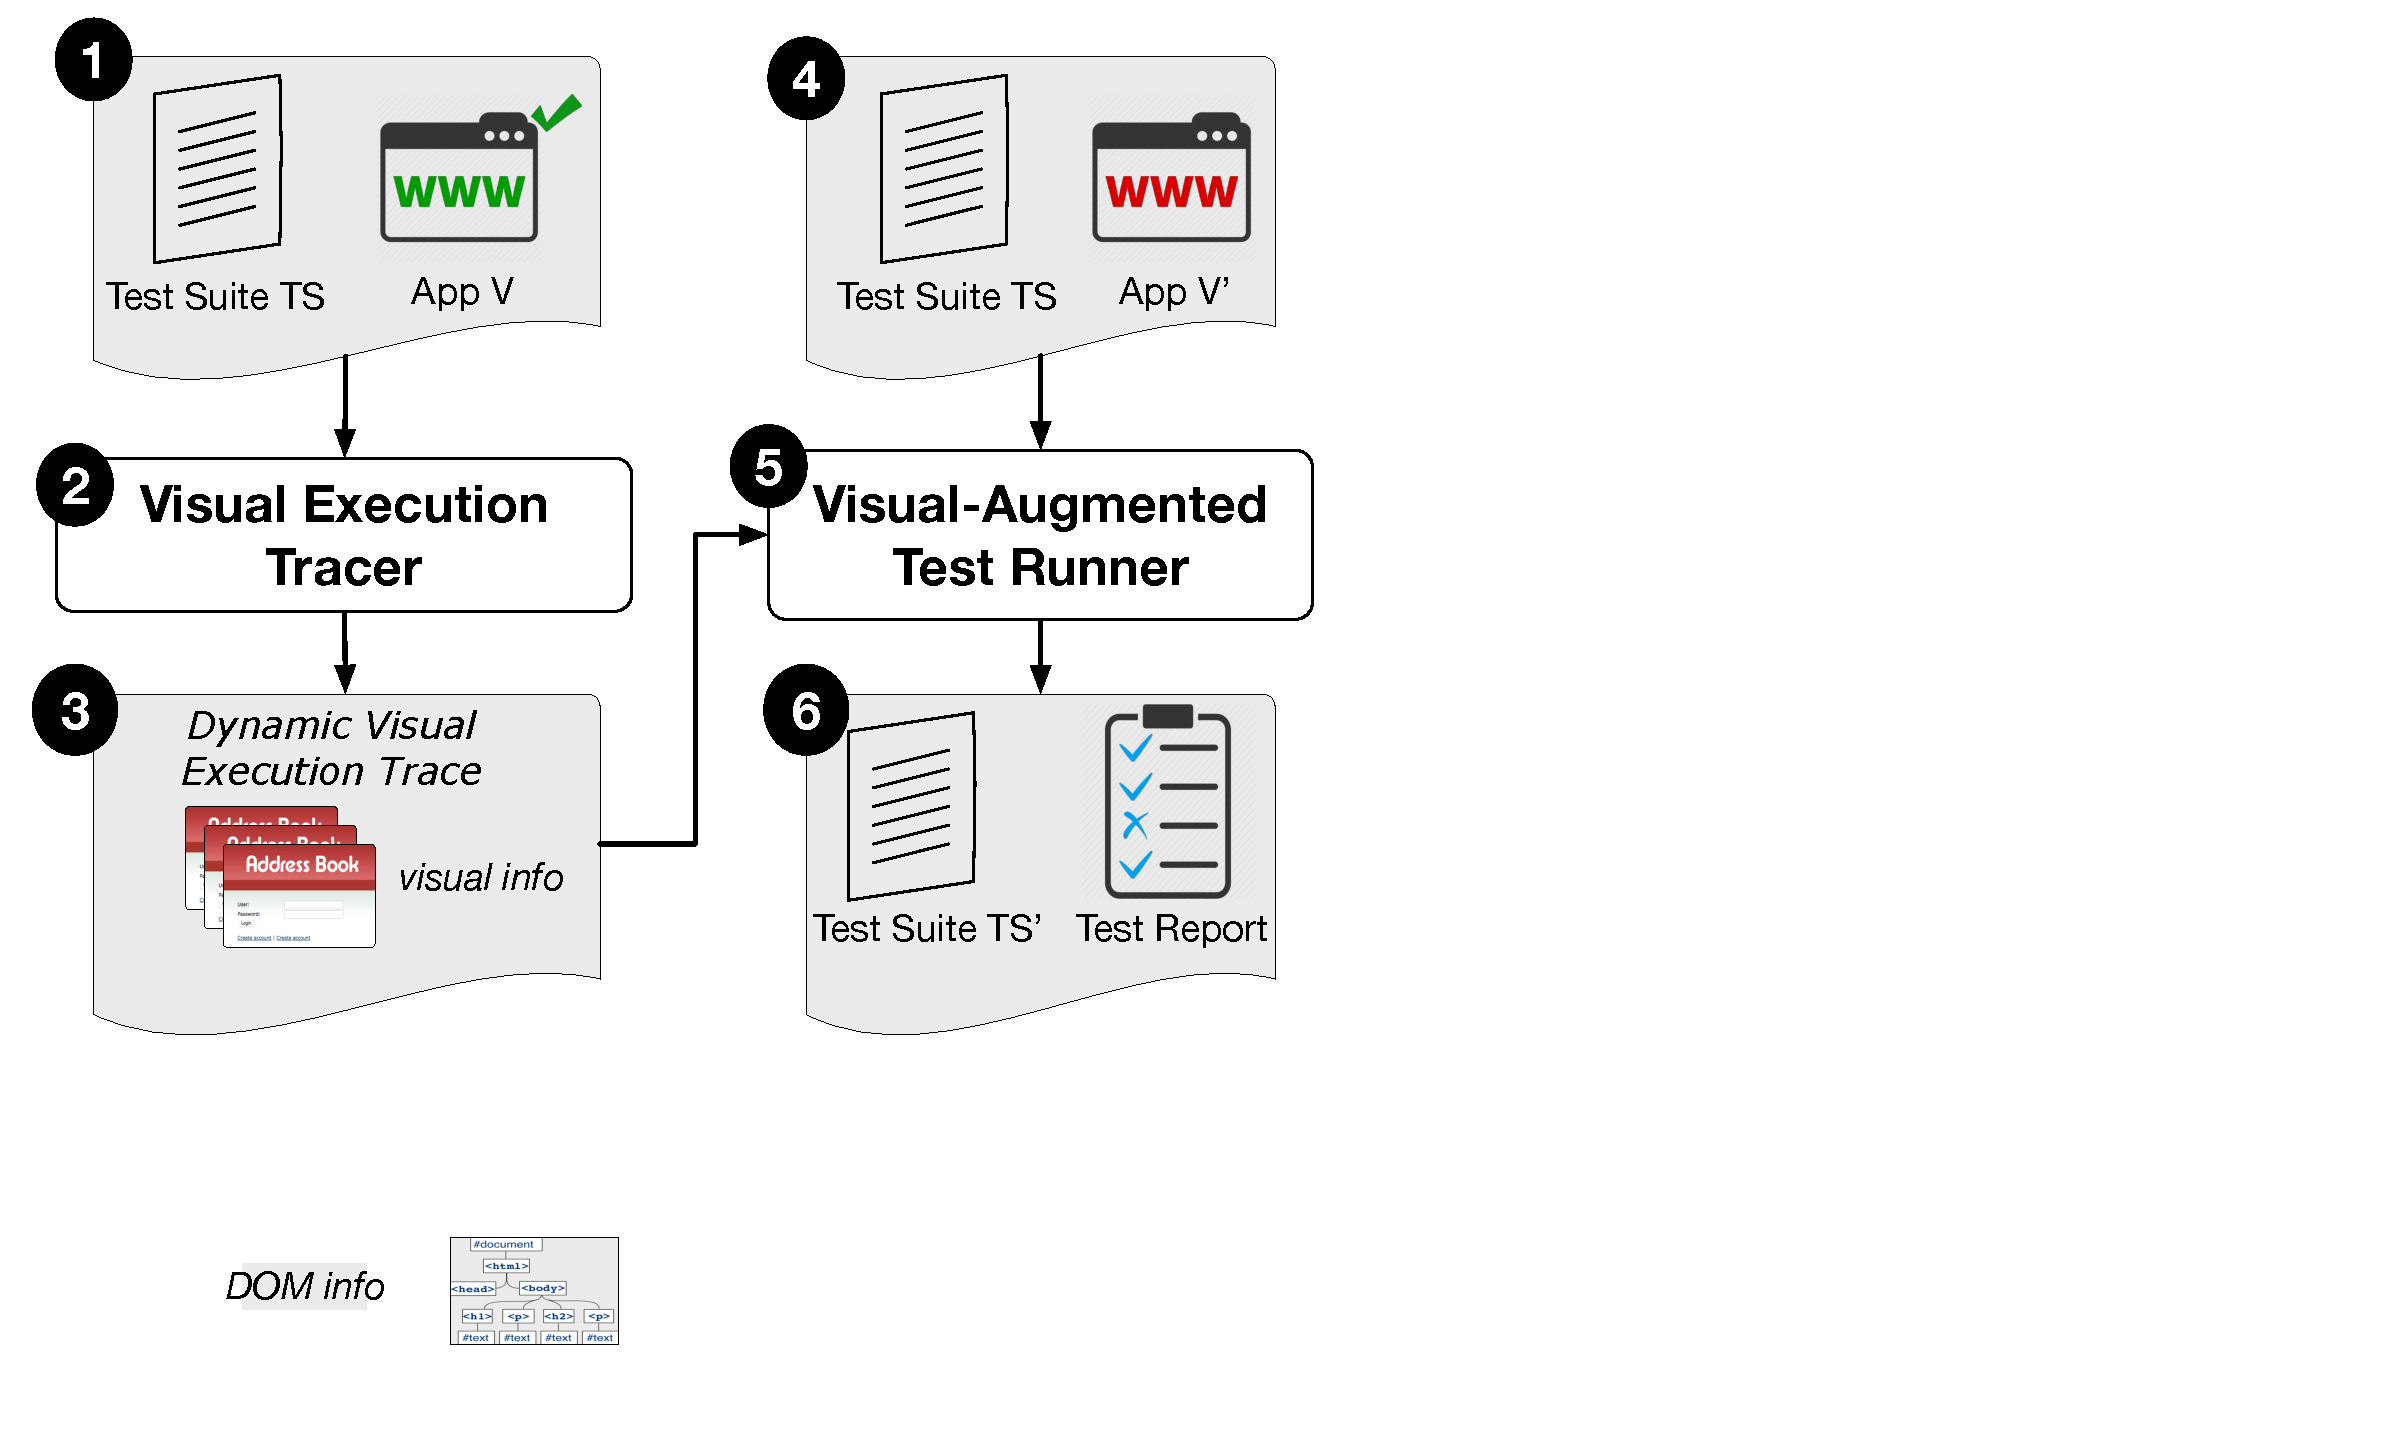
\includegraphics[trim={0.2cm 6.5cm 17cm 0.2cm},clip,scale=0.26]{images/approach-bigger}
%}
\caption{Overview of our approach. Inputs and outputs are shown as parallelograms, whereas the proposed approach is represented as rounded rectangles. \andrea{T -> TS}}
\label{approach}
\end{figure}

\autoref{approach} illustrates the usage scenario for our approach in a real-world testing environment. 
First, given a stable version of the web application $V$ along with its working test suite $TS$ (i.e., in which all tests pass)~\ding{182}, a tester would run $TS$ by means of the first module of the presented approach~\ding{183}. Such a module collects, for each test, a variety of information (e.g., screenshots, DOMs)~\ding{184}. 
Then, as the application $V$ evolves into a new version $V'$ ~\ding{185}, a tester may wish to use $TS$ to check if regressions have occurred. Here, the tester uses the second module of our approach~\ding{186} which runs each test case of the the test suite $TS$ against the new version $V'$, and makes use of the information about the previous execution traces to verify the correctness of each test statement, and eventually attempt to repair locator breakages at runtime in an \textit{online mode}. At the end of the process, the approach outputs the new verified \andrea{dangerous word} (and eventually repaired) test suite $TS'$ that works on $V'$, together with report information. 
The developer/tester can then manually analyze the report along with repairs that were automatically performed as well as suggested repairs to create an evolved test suite $TS'$. The test suite $TS'$ represents a working test suite for the version $V'$ which can be used in the same way when $V'$ evolves. 
The manual effort required is potentially significantly reduced in comparison to a user carefully verifying each executing test and manually searching for fixes as breakages occur. %
We now detail each step of our approach. 

\subsection{Execution Trace Collection}
%
In the first part of our approach, we capture a model of the  runtime execution of the test cases. 
The test model is a sequence of test states, where each test state captures the DOM and visual information associated with each test statement of each test case. 

%While most of the DOM information could be collected statically, the visual appearance of the rendered elements may change during the application execution and some elements may be not visible until specific events occur. For this reason, we need to capture the visual information at runtime, while the test suite is executing. 

%To this aim, the first module of \tool takes as input a web application along with its accompanying test suite, and runs each test case to collect both DOM and visual information associated to each test statement, hence creating a test model.  %\andrea{I haven't detailed this part by means of an algorithm as references are provided}

%We used and adapted the publicly available version of \textsc{PESTO}~\cite{2014-Stocco-SCAM}, a tool that uses aspect-oriented programming~\cite{aop} -- to intercept all Selenium WebDriver method calls (e.g., \texttt{click()}, \texttt{sendKeys()}, etc) using properly defined join-points. 

%We use aspect-oriented programming~\cite{aop} to intercept all Selenium WebDriver method calls (e.g., \texttt{click()}, \texttt{sendKeys()}, etc) using properly defined join-points. When a given join-point matches, advice methods store the test state \textit{before} and \textit{after} the statement's execution. 

The test state encompasses the following DOM-related information: \textit{(d1)}~the complete HTML page, \textit{(d2)}~the DOM, \textit{(d3)}~the XPath of the web element the test statement interacted with and \textit{(d4)}~all its HTML attributes. The collected visual information concern: \textit{(v1)}~the screenshots, \textit{(v2)}~the coordinates and size of the web element's bounding box, and \textit{(v3)}~a visual locator for it. A visual locator is the portion of the rendered web page that uniquely identifies such web element on the screen. (Note that, as explained in~\cite{2014-Stocco-SCAM,2015-Leotta-SAC}, a visual locator is not always the precise crop of the web element's bounding box. There are cases in which a larger crop -- taking into account the web element's visual context --  is necessary in order to visually differentiate it from other visually similar web elements appearing on the page, as the case of a list of input text fields in a form).

We refer to this model of the runtime execution of the tests as \textit{dynamic visual execution trace}. \andrea{name}

\subsection{Visual-Augmented Test Suite Runner}

\autoref{algo:alg1} illustrates the main procedure of our algorithm for the visual-augmented execution of test cases. The procedure takes as input the execution trace $EX$ of a test case $T$ on version $V$ of the web application, the test case $T$, and the URL $U$ of the web application $V'$. The outputs are a test $T'$, and a list of verified/repaired statements. 

\textbf{Initialization.} 
The initial part involves loading the previously saved trace execution information of the test $T$ on the reference version $V$, and loading the new version $V'$ by means of Selenium WebDriver (Lines~1--2). 

\textbf{Visual-Augmented Execution.}
Such information is used to ``visually'' validate each statement $st_i$ of $T$, when executed on $V'$ (main loop Lines~4--36). The validation proceeds as follows. First, the DOM-based locator utilized by the test statement is extracted from $st_i$, along with the visual locator (e.g., an image) and the DOM information associated to the trace of $st_i$ in $V$  (Lines~5--7). Then, the \texttt{driver} instance is used to query the DOM of $V'$ to observe if the locator returns a web element (Line~8). 

\begin{algorithm}[b]
\scriptsize
\DontPrintSemicolon % Some LaTeX compilers require you to use \dontprintsemicolon instead
\KwIn{$T$: A test case developed for web application $V$, the URL $U$ of its subsequent version $V'$, $EX$: Execution Trace of $T$ when executed on $V$}
\KwOut{$T'$: A verified/repaired $T$ working on $V'$}
%\colorbox{lightgray}{/* Execution Trace collection */} \;
\textit{trace} $\gets$ loadExecutionTrace($EX$) \;
\textit{driver} $\gets$ loadApp($U$) \;
\textit{statements}, \textit{repairedStatements} $\gets$ getStatements(T) \;
 \ForEach{ test statement $st_i \in$ \textit{statements} }{%
  \textit{locator} $\gets$ getLocator($st_i$)\;
  \textit{\textit{visLocator}} $\gets$ getVisualLocator(\textit{trace}, $st_i$) \;
 \textit{\textit{DOMInfo}} $\gets$ getDOMInfo(\textit{trace}, $st_i$) \;
  \textit{webElement} $\gets$ \textit{driver}.findElement(\textit{locator})\;
  \HiLi{/* Manage non-selection of web element. */} \;
   \uIf{webElement == null} { 
     \textit{webElemVisual} $\gets$ \textsc{visualSearch}(\textit{driver}, $st_i$, \textit{visLocator}, \textit{DOMInfo})\;
     \uIf{\textit{webElemVisual} == null} {
       \textit{webElemVisual} $\gets$ \textsc{localCrawling}(\textit{driver}, $st_i$, \textit{visLocator}, \textit{DOMInfo})\;
       \uIf{\textit{webElemVisual} == null} {
       \textit{repairedStatements}.remove($st_i$)\;
       } \Else{
       \textit{newStmt} $\gets$ <\textsc{synthetizeLocator}(\textit{webElemVisual}), ``click'', ``''> \;
       \textit{repairedStatements}.addBefore($st_i$, \textit{newStmt}) \;
        }
     } \Else{
     updateLocator($st_i$, \textit{webElemVisual}) \;
      \textit{repairedStatements}.update($st_i$) \;
     }
   \HiLi{/* Manage mis-selection of web element. */} \;
   } \ElseIf{webElement $\neq$ null}{
      \textit{webElemVisual} $\gets$ \textsc{visualSearch}(\textit{driver}, $st_i$, \textit{visLocator}, \textit{DOMInfo})\;
     \textit{webElement} $\gets$ \textsc{verify}(\textit{webElement}, \textit{webElemVisual})\;
      \textit{repairedStatements}.update($st_i$, \textit{webElement}) \;
   }
   \HiLi{/* Suggest potential fix to assertions value. */} \;
    \If { webElement.getText() $\neq$ getTextualContent($st_i$) } {
         \textit{newStmt} $\gets$ <\textit{webElement}, ``getText'', webElement.getText()> \;
      	\textit{repairedStatements}.replace($st_i$,  \textit{newStmt}) \;
      }
         \textit{driver} $\gets$ \textsc{executeStatement}($st_i$, $V'$) \;
      	$T'$.add($st_i$) \;
 }
\Return{$T'$, \textit{repairedStatements}}\;
\caption{Overall Algorithm}
\label{algo:alg1}
\end{algorithm}

\textbf{Detecting and Repairing non-selection problems.}
If no elements are returned, we treat it as a non-selection, and $st_i$ will break in $V'$, which we attempt to repair through a series of countermeasures. The first heuristic tries to search for the web element \textit{visually} on the same state. The \texttt{visualSearch} function (Line~11) uses advanced computer vision algorithms to retrieve the target web element visually by  matching the visual locator captured in $V$ on the current screenshot of $V'$. The DOM information is also used to guide the search, and filter out potential outliers or visual false positives (such as visual duplicates). If a result is found, the locator of $st_i$ is updated, and the corrected statement saved in the list of repairs (Line~21--22). Then, $st_i$ is executed, and saved as a statement of the new test case $T'$ (Lines~34--35), before proceeding to the next statement.

\begin{figure*}[t]
\centering
%\fbox{
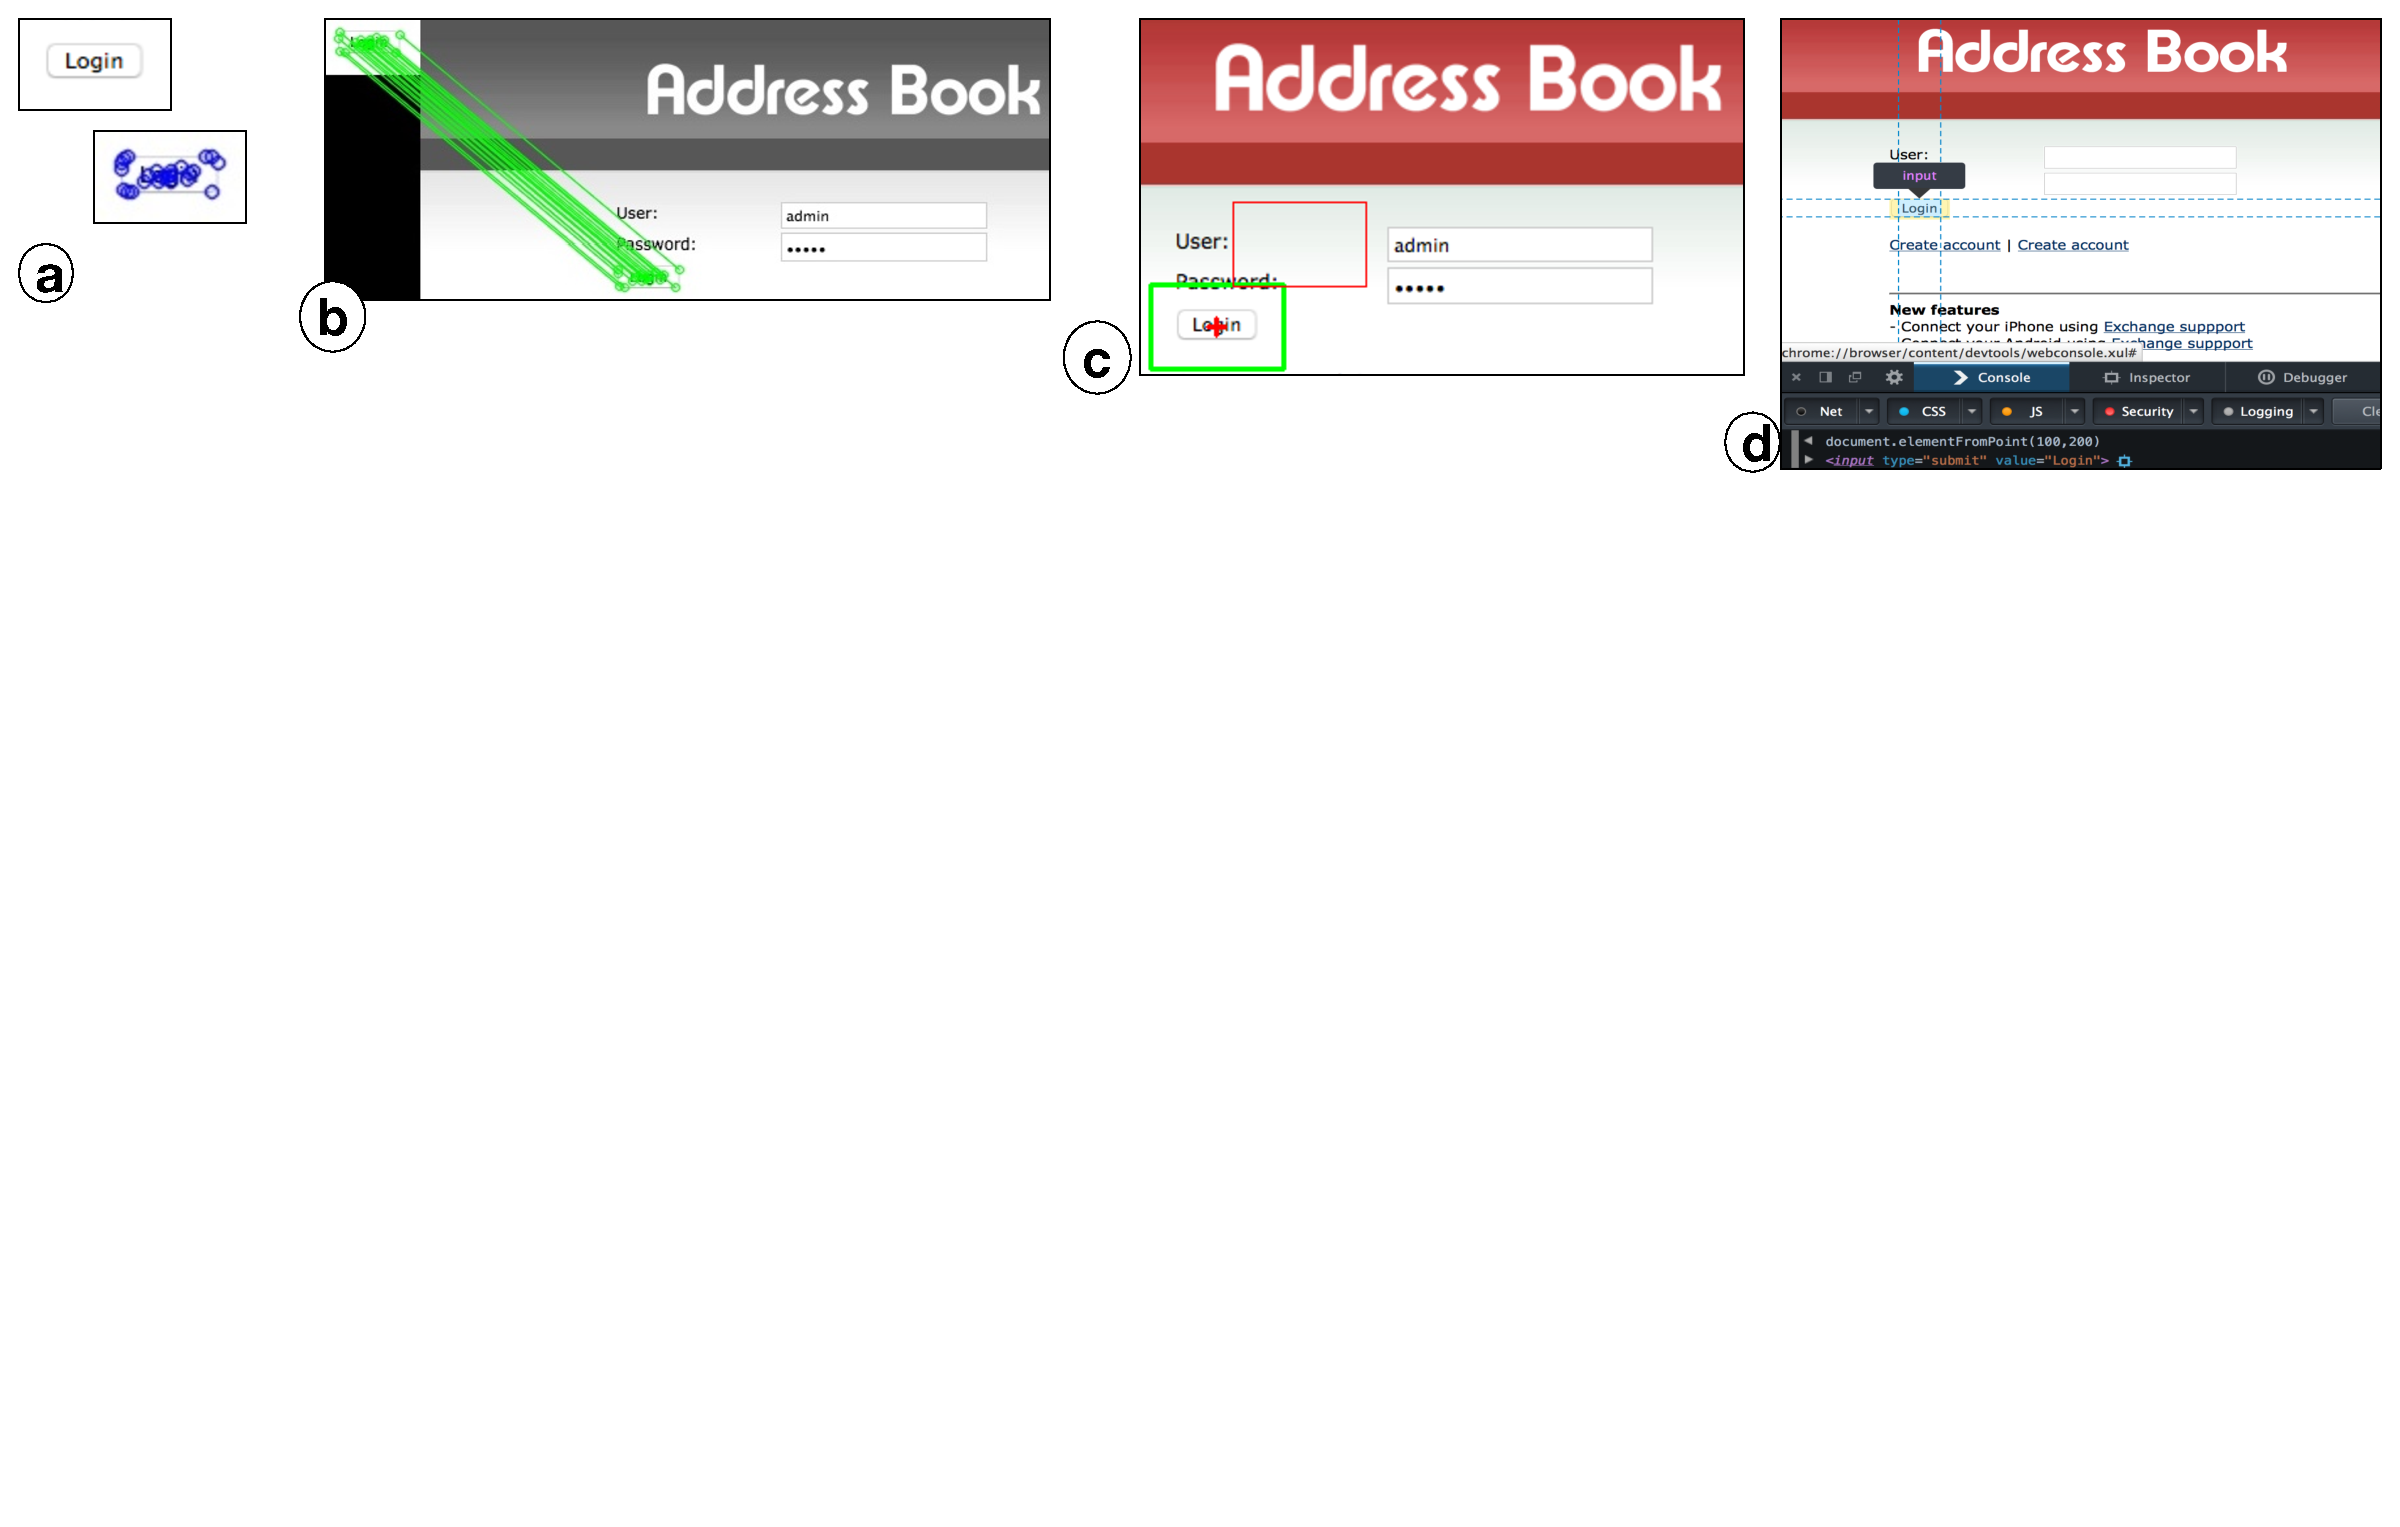
\includegraphics[trim={0.3cm 17cm 0.4cm 0.3cm},clip,scale=0.44]{images/cv}
%}
\caption{Computer vision pipeline for robust web element detection.}
\label{fig:cv}
\end{figure*}

If the visual search on the same state fails, then our approach assumes that the element no longer exists on the current state. We consider this a broken workflow and trigger a local exploration of the application state space (procedure \textsc{localCrawling} of Line~13) in order to find the element in the neighbouring states. In each new state discovered by the exploration, we attempt the \textsc{visualSearch} procedure to locate the element. If a match is found in at least one of those states, a new statement to reach that state (i.e, page) is created, with the corresponding DOM locator, and a default \texttt{click} action, and added before $st_i$ in the the list of repairs (Lines~17--18). (We currently do not support the creation of general purpose statements, such as the ones that need input data).

On the contrary, if a match is not found, i.e. we cannot locate the element through local crawl, we attempt to repair the broken workflow by deleting the $st_i$ and proceeding to the next test statement (Line~15).

\textbf{Detecting and Repairing mis-selection problems.}
If a web element was returned by the initial DOM-based locator, our approach asserts the correctness of the selection by using the previously collected visual and DOM information (Lines~25--33). Additionally, in case of assertions, if the GUI textual information of the web element has changed, a new statement with the potentially corrected assertion is created and saved in the list of repairs (Lines~29--33). \andrea{suggestion?}
Note that we only suggest a repair to the assertion statements but do not attempt to repair them automatically since only a human tester upon manual inspection can ascertain whether a new value in GUI reflects the intended application behaviour.
Thus, the execution of $st_i$ will likely raise an \texttt{AssertionError} for the tester to inspect, for which a candidate repair has been automatically created.

\textbf{Outputs.}
If \autoref{algo:alg1} terminates, our approach was able to either correct all the statements of $T$ or provide suggestions for it. 
% in the new version $V'$. 
 If $T = T'$ no regressions have occurred, otherwise the list of repairs is returned.
If \autoref{algo:alg1} stops prematurely, then one of the statements executed by the function \textsc{executeStatement} triggered an action that could not be performed or an incorrect locator was retrieved. The tester must then intervene to manually correct such unfortunate cases.

In the following sections we describe the core components of our algorithm, that is the \textsc{visualSearch} and \textsc{localCrawling} procedures that underlie at the functioning of our approach.

\subsection{Visual Search of Web Elements}

As described in \autoref{sec:cv}, matching specific portions of images across different versions of a web application is a challenging task, for which existing computer vision (CV) algorithms perform poorly. 

Thus, the \textsc{visualSearch} adopts a pipeline of CV algorithms, each one devoted to a specific task. The pipeline is graphically illustrated in \autoref{fig:cv}. In the first step, we need to robustly detect the absence/presence of the template image in the screenshot. As anticipated in \autoref{sec:tm}, pure template matching is not adequate. % for this problem. 

\textit{Feature Detection for Template Absence/Presence.}
We adopted two famous feature detection algorithms from the CV literature, SIFT~\cite{Lowe1999,Lowe2004} and FAST~\cite{rosten2005tracking,rosten2008faster}, to detect the key-points from the template image~\textcircled{\raisebox{-0.6pt}{a}}. Through experimentation, we found that these two approaches complement each other well and applying both of them together is beneficial. SIFT performs well mostly for text-based templates whereas FAST can handle the cases where the template represents an ``empty'' text field, as it is specifically designed for corner detection. In our pictorial example~\textcircled{\raisebox{-0.6pt}{a}}, most of the key-points detected by SIFT are in fact nearby the ``Login'' label, whereas FAST detected key-points also in proximity of the corners.
 
Then, descriptors are calculated for each key-point, and the algorithms try to match them onto the new screenshot~\textcircled{\raisebox{-0.6pt}{b}}.
If at least 70\% of key-points are matched across the two images, we can have a certain degree of confidence that the template is present in the image. 

\textit{Template Matching with visual and DOM filtering.}
In the next step, if the feature detection returned true, a pure template matching technique is executed~\textcircled{\raisebox{-0.6pt}{c}}. The performance of template matching oscillate depending on various factors, such as the size, and the threshold being used. For this reason, the templates that do not fall in the region where most of the key-points have been found, are discarded (\textit{visual-based filtering}). If multiple matches are still present, we retrieve the DOM elements corresponding to each match, and we calculate the closest web element that matches the DOM information (\textit{DOM-based filtering}).
Thus, only the closest match is returned (see the green thick rectangle over the ``Login'' button). In brief, the three algorithms operate to find a consensus on the area in which the best match can be found. 

\textit{From GUI to DOM.}
To retrieve the DOM-element corresponding to a specific point of coordinates $(x,y)$, \textsc{visualSearch} queries the browser through a JavaScript command -- \texttt{elementFromPoint(x,y)} -- that returns the DOM element whose bounding box contains \texttt{x} and \texttt{y}. 

%To precisely identify the web element of interest, we need to provide the function with the coordinates of the the \textit{centre} of the bounding box. Otherwise, a DOM ancestor of the searched web element (e.g., the \texttt{form} container), will be erroneously retrieved.

\subsection{Local Crawling for Workflow Repair}

Manually repairing every broken workflow is tedious and frustrating, since even a medium-size web application may contain tens of GUI screens and hundreds of GUI actions. It is hence likely infeasible for a tester to quickly explore this space to choose replacement actions from.

Fortunately, a web crawler can do this automatically. To this end, the \texttt{localCrawling} function integrates \textsc{Crawljax}, a state of the art tool for the automatic crawling of dynamic web applications~\cite{mesbah:tweb12,mesbah:tse12}. We developed a \textsc{Crawljax} plugin that incorporates the \texttt{visualSearch} function (Line~11), so that the crawler can effectively explore the state space of $V'$ looking for a visual match in all the neighbouring states of the current test state (Line~13). As a conservative choice, since the number of DOM states and events can be numerous, we set the crawling depth to one (1). On the one hand, this limits the search capability, potentially missing states in which the elements could be found. On the other hand, this choice keeps the running time acceptable.

\subsection{Implementation}\label{sec:implementation}

We implemented our approach in a tool called \tool, which is publicly available (URL omitted). 
The tool is written in Java, and supports Selenium test suites written in Java. However, our overall approach is more general and applicable to test suites developed using other programming languages or testing frameworks. 
\tool gets as input the path to the test suites, collects the visual execution traces by means of \textsc{PESTO}~\cite{2014-Stocco-SCAM}, runs the visual-augmented detection and repair algorithm using the computer vision libraries available in OpenCV~\cite{}, and \textsc{Crawljax} for the local crawling exploration. 
\tool makes use of the traces to generate potential repairs and generates a list of repaired test cases.








% !TEX root =  paper.tex

\section{Empirical Evaluation}\label{sec:evaluation}

We consider the following research questions:

\noindent
%\textbf{RQ\textsubscript{1} (detection):} How effective is our proposed visual-aided approach in visually verifying test statements?
%\textbf{RQ\textsubscript{1} (prevalence):} How prevalent are test breakages in practice?

\noindent
\textbf{RQ\textsubscript{1} (repair):} How do DOM-based and visual-augmented test repair approaches compare in terms of effectiveness?

\noindent
\textbf{RQ\textsubscript{2} (running time):} What is the running time of executing our visual-augmented approach as compared to the DOM-based one? \\

%\noindent
%\textbf{RQ\textsubscript{4} (duration):} Does \tool decrease the duration of web test repair tasks?
%
%\noindent
%\textbf{RQ\textsubscript{5} (accuracy):} Does \tool increase the accuracy of web test repair tasks? \\

\noindent
The repair strategy of \tool can be customized so as to utilize: (i)~only DOM-based information, (ii)~only visual-based information,  (iii)~both DOM-based and visual information. We refer to these three variants as \tool-DOM, \tool-Vis, and \tool-Hybrid, respectively.
%In our study, the visual-augmented approach is represented by \tool, and the DOM-based approach is represented by \water. 
%RQ\textsubscript{1} aims at evaluating how effective the three variants of \tool are at detecting and repairing test breakages. 
% the correctness of the test statements or signalling the occurrence of a breakage, and how its effectiveness varies across breakage classes. 
%RQ\textsubscript{1} and RQ\textsubscript{2} aim at comparing our proposal against the state of the art web testing repair solution under different effectiveness and efficiency measures. Finally, we aim at evaluating whether the tool can effectively aid humans in detecting and repairing test breakages, as compared to a manual fashion.
Thus, RQ\textsubscript{1} and RQ\textsubscript{2} aim at comparing the effectiveness and efficiency of the three variants of our approach.

\subsection{Procedure}\label{sec:procedure}

Then, for each subject applications, we applied the three variants of our approach to each $(T_n,V_{n+1})$ pair in which either a breakage or a failure has been observed. For each variant, we ran the repaired test $T_{rep}$ to determined whether the tool was able to detect (and possibly repair) the issues. If $T_{rep}$ executed and passed, we counted the number of breakages that were \textit{corrected} (true positives). If $T_n$ failed because of a bug, and $T_{rep}$ was able to report it, we counted the number of correct \textit{detections} (true negatives). Conversely, the false negatives are represented by \textit{missed} detections or \textit{incorrect} repairs. False positives occur when our approach signalled a breakage or a failure, even if the statement is actually correct.


\subsection{Threats to Validity}\label{sec:ttv}

\head{Internal validity} We limited the bias of having produced test suites ourselves, that could constitute a threat to the internal validity of our work, by choosing existing test suites used in the previous web testing research. This also ensures, to some extent, that the chosen object of analysis are non-trivial, therefore representative of a test suites that a real web tester would implement. 

\head{External validity} Concerning the generalizability of our results, we ran our approach with a limited number of subjects and test suites. However, we believe the approach to be applicable in a general web testing scenario, even though the magnitude of the results might change when considering different test suites and applications. To limit biases in the manual selection of the versions, we considered \textit{all} the available releases after those for which the test suites were developed for.
 

%\textit{Procedure and Metrics.}
%
%For each considered application: 
%
%\begin{itemize}
%\item we executed each test suite $T_k$ created for a version $V_k$ by means of the Visual Trace Generator, which collected information about the tests execution (e.g., DOMs, screenshots, etc);
%\item we ran each $T_k$ on the next version $V_{k+1}$ with the Visual Test Suite Runner and collected information about each detection, breakage, automatic as well as manual repair triggered.
%\end{itemize}
%
%\noindent
%To answer RQ\textsubscript{1} (\textbf{detection}), we counted the number of statements that were correct, and that our technique was able to visually verify. Those cases represent the true positives (TP\textsubscript{detection}). On the other hand, if our tool deemed those cases as incorrect (i.e., was not able to verify them), then they represent the false negative FN\textsubscript{detection}. Conversely, if the statements were broken, and our technique detected the breakages, we counted them as true negative TN\textsubscript{detection}, whereas if the tool deemed them as correct, then is a false positive FP\textsubscript{detection}.
%%
%In the case of FN and TN, \tool attempts a repair. We also counted the number of correct (REP\textsubscript{correct}) and wrong repairs (REP\textsubscript{wrong}). (Note that in the FN cases, repairs were unnecessary (REP\textsubscript{unnecessary})). Moreover, to fully evaluate the limitations of our technique, we counted the statements that were repaired manually (REP\textsubscript{manual}) and the statements that were found to be unrepairable both by manually and automatically (REP\textsubscript{unrepairable}).
%
%\noindent
%To answer RQ\textsubscript{2}, we counted the number of tests that \tool and \water were able to repair.
%
%\subsection{Study 2}
%
%We designed a user study to measure how effective the tool is in the identification of the root cause, and how much time it allows to save.

\subsection{Results}\label{sec:results}












% !TEX root =  paper.tex
\section{Discussion}\label{sec:discussion} 

In this section, we discuss some of our evaluation findings, tool design decisions and limitations, as well as threats to validity of our study.

\head{Prevalence} Our empirical study confirmed the findings of previous studies about the fragility of E2E web tests when used for regression testing scenarios (\autoref{sec:taxonomy}). 
Although such tests did fail 94 times due to actual bugs, the number of breakages (733) is still predominant. 329/2672 tests of our benchmark (12\%) experienced at least one breakage that the test engineer must inspect, and find an appropriate repair for. 

\head{Automatic Repair} 
Our evaluation revealed that \tool can repair more than 80\% of the total number of breakages correctly. Therefore, we believe our algorithm and its heuristics to be accurate in the repair task.

We investigated why \emph{all} breakages were not repaired. We enumerate some of the main reasons next, which pertain to both the inherent nature of our subjects and tests and some of design choices of the two competing approaches. 

Our results highlighted that \water cannot repair any Mis-Selection breakage (\textit{Scenarios~4 and~5}). This is motivated by the intrinsic design of the DOM-based algorithm. Indeed, one of the repair heuristic of \water attempts to search the target web element by its XPath in the new evolved DOM. If an element is found, then \water returns a wrong element. \tool, on the other hand, does not trust \textit{a priori} DOM-based locators and validates them by means of their visual appearance. This is why our solution could detect and repair $\approx$83\% of the \textit{Mis-Selection} cases. 

For analogous reasons, the DOM-based repair strategy of \water was ineffective when searching elements with local crawling (\textit{Scenario~2}). \tool could detect nearly one third of such cases. The failing cases were mostly due to the retrieving of no elements (or wrong ones). In PPMA, a challenging case occurred: the desired element was hidden in a hoverable dropdown menu, whereas the crawler is designed to search for the web element in the neighbouring states. Moreover, our tool currently does not support the creation of general purpose statements, such as the ones that need input data. %This leaves room for improvement. 

Concerning the elements being removed (\textit{Scenario~3}), both techniques failed in seven cases because the crawling phase did retrieve a wrong element. 
\textit{Scenario~1} represents the most common class of breakage, and both the techniques perform quite well. However, \tool had a $33\%$ increase in the correct repair rate. Only in three cases (for Claroline application), \water was able to find a correct repair when \tool was not. This was due to `edit' buttons whose DOM attributes were stable across the two considered releases whereas their visual appearance did change making our visual technique ineffective.

Looking at the results on a per-application basis, AddressBook and Collabtive tests experienced breakages pertaining to all classes. 
\tool performed better than \water, with 165\% and 11\% increment on the number of correct repairs, respectively. 
For AddressBook, the DOM gets evolved quite frequently across the releases. Thus, for a tester would be challenging to find reliable attributes upon which to create stable web elements locators  (and hence robust test suites). Also the GUI of the web application gets evolved as changes in background colour and font size to make it more appealing and user-friendly. However, our approach demonstrated to be robust to both shifting and scaling (invariant to translation and scale transformation). 
%
There are five mis-selection breakages that could not be corrected by either of the two approaches. Those cases refer to again `edit' buttons whose position in the DOM and visual appearance did change substantially. 

Collabtive is the application in which both techniques have their best performance. Indeed, both the DOM and the GUI remained quite stable across the analyzed releases. The high number of breakages is explained by the numerous XPath locators used in the test suite, which make them fragile to minor DOM changes. However, such modifications at a DOM level did not jeopardize the applicability of \water.

For Claroline and PPMA web applications, almost the entirety of the breakages refers to \textit{Scenario~1}, with \tool being 134\% and 17\% more effective than the DOM-based repair, respectively. Those applications are the ones in which more manual repairs were needed. Claroline experienced both major DOM and GUI evolutions, whereas in the case of PPMA our technique had problems with timing issues (e.g., delays or page reloads that were needed to display the web elements on the GUI).

\head{Performance and Overhead} 
On average, \water was nearly three times slower than \tool mainly for two reasons: (1)~if the target element was still on the same state, and the heuristics failed to find it, the crawler was unnecessarily executed, and (2)~one of the heuristics searches for web elements having \textit{similar} XPaths. In our applications, the DOM size can be quite big, and \water is often forced to elaborate the similarity on dozens of elements. On the contrary, \tool adopted advanced image-processing algorithms, which requires one single template matching operation on images of reasonable size (i.e., screenshots of web pages).

On the whole, we believe that the potential benefits outweigh the foreseeable overhead given (1)~our results in the automated repairs, and (2)~the speed of our image processing pipeline. However, should strict time constraints apply, the pre-processing step (Visual Execution Tracer) can be carried out overnight.

Manually inspecting the application to find a candidate repair  and create a locator for \textit{each} broken statement can be in fact quite time-consuming. Our own experience in repairing tests, which we were required to do while devising \tool, corroborates the costliness of the task. For example, in AddressBook, one of the test for the search functionality fails 11 times when applied from version 4.02 to version 4.1.1: three elements gets removed (\textit{Scenario~3}) and seven mis-selections occur (\textit{Scenario~4}). \tool created the dynamic visual execution trace of the test in 22~s, and then it found correct repairs for all 11 breakages in $\approx$57~s. Thus, in this specific case, our technique can have prospect for success if the manual detection and repair performed by a human tester is lower than 80~s. However, empirical studies with human subjects are necessary to measure the costs associated with repairs. Before incurring in such expense, we evaluated whether out technique has prospect for success against the state of the art algorithm.

\head{Applications} 
\tool can be used by test engineers to validate and repair their E2E web test cases. Each statement of the tests is associated with their visual trace information. Hence, this can aid testers to perform more effective \textit{root cause analysis}.

Alternatively, our technique can play a role in \textit{automating software oracles}. A similar approach is implemented in Applitools~\cite{applitools}, where testers can manually inject visual checks at specific places of the test's execution. This has two drawbacks: (1)~the insertion of the check-points must be performed manually, (2)~this extra-code clutters the initial test code, with statements that do not pertain to the test scenario itself. On the contrary, our technique can be introduced smoothly in the testing team, because it requires no modification at the source code level. 

Finally, \tool can be utilized as a \textit{runtime monitoring}  technique for the detection of breakages tests. We have demonstrated that \tool goes beyond simple detection and can efficiently correctly most of the breakages at runtime, hence it is a first step towards automated \textit{self-repair} testing techniques. 

\head{Threats to Validity}\label{sec:ttv}
We limited the bias of having produced test suites ourselves, that could constitute a threat to the internal validity of our work, by choosing existing test suites used in the previous web testing research. This also ensures, to some extent, that the chosen object of analysis are non-trivial, therefore representative of a test suites that a real web tester would implement. 
%
Concerning the generalizability of our results, we ran our approach with a limited number of subjects and test suites. However, we believe the approach to be applicable in a general web testing scenario, even though the magnitude of the results might change when considering different test suites and applications. To limit biases in the manual selection of the versions, we considered \textit{all} the available releases after those for which the test suites were developed for.
\section{Related Work}\label{sec:relwork}



There exist a body of knowledge describing the kind of repair activities that a tester must perform during test suites maintenance. 

\head{Web Test Repair} \textit{Choudhary et al.}~\cite{Choudhary:2011:WWA:2002931.2002935} distinguish three main reasons for tests scripts to break: (1)~structural, (2)~content, and (3)~blind. The first category concerns DOM elements that get repositioned in the tree due to node/attribute insertion, modification or deletion. The second category concerns the textual content that get updated during software evolution. At last, the third category is related to server-side changes that are not directly observable in any DOM modification, such as popup boxes. 
%
In a recent work, \textit{Hammoudi et al.}~\cite{Hammoudi-2016-FSE}, an incremental test repair approach called \textsc{WaterFall}, has been proposed. Test repair techniques are applied iteratively across a sequence of fine-grained versions of a web application. Results of an empirical study comparing \textsc{WaterFall} to a coarse-grained approach (\textsc{Water}) show that the former is more effective than the latter at automatically repairing tests.
%
\textit{Leotta et al.}~\cite{2015-leotta-ICST} suggest to go beyond the concept of single locator and propose and experiment with a set of equivalent locators, called multi-locator. 
%Locators are resilient to different types of changes and tend to be fragile individually, not collectively. 
The idea is to compensate for one locator's fragility by resorting to the capabilities of another locator. Despite the improvement from the robustness point of view, the locator repair algorithm is also able to perform the correct repairs of the locator set in most of the cases, by relying on the redundancy of set of locators.

\head{Test Case Breakages}  
\textit{Hammoudi et al.}~\cite{Hammoudi-2016-ICST} present a taxonomy of web breakages in the context of record/replay tests. At a high level, they distinguish between proximal and distal causes. They define a proximal cause of a breakage as the cause which is most closely related to that breakage. Distal causes, on the other hand, are the modification that are made on the web application during its natural evolution and/or maintenance. For instance, the fact that a developer removes a choice from a dropdown list is a distal cause; the fact that a test fails at localizing that missing element is the proximal cause for which a tester must find an appropriate repair. 
%
In another paper, \textit{Leotta et al.}~\cite{2016-leotta-Advances} distinguish between \textit{structural} changes and \textit{logical} changes. The former involve the modification of the web page structure (i.e., the DOM) that impact only the low-level test script statement associated with that page and modification. The latter category, on the other hand, involve a change of the test scenario for which one or more test statements need to be added, altered or deleted.





\begin{enumerate}
%\item \textst{Choudhary WATER}
%\item \textst{WATERFALL}
\item Ernst workflow
\item Atif SITAR
\item ROBULA (locator breakage prevention)
%\item \textst{Multilocator (locator breakage prevention and repair)}
\end{enumerate}

% !TEX root =  paper.tex
\section{Conclusions and Future Work}\label{sec:conclusions}

\begin{itemize}
\item detect silent breakages
\end{itemize}



\balance
%\bibliographystyle{ACM-Reference-Format}
\bibliographystyle{acm}
\bibliography{paper}

\end{document}
